\documentclass[a4paper,UKenglish,cleveref,autoref,thm-restate,numberwithinsect]{lipics-v2021}
%This is a template for producing LIPIcs articles. 
%See lipics-v2021-authors-guidelines.pdf for further information.
%for A4 paper format use option "a4paper", for US-letter use option "letterpaper"
%for british hyphenation rules use option "UKenglish", for american hyphenation rules use option "USenglish"
%for section-numbered lemmas etc., use "numberwithinsect"
%for enabling cleveref support, use "cleveref"
%for enabling autoref support, use "autoref"
%for anonymousing the authors (e.g. for double-blind review), add "anonymous"
%for enabling thm-restate support, use "thm-restate"
%for enabling a two-column layout for the author/affilation part (only applicable for > 6 authors), use "authorcolumns"
%for producing a PDF according the PDF/A standard, add "pdfa"

\pdfoutput=1 %uncomment to ensure pdflatex processing (mandatatory e.g. to submit to arXiv)
\hideLIPIcs  %uncomment to remove references to LIPIcs series (logo, DOI, ...), e.g. when preparing a pre-final version to be uploaded to arXiv or another public repository

%\graphicspath{{./graphics/}}%helpful if your graphic files are in another directory

\bibliographystyle{plainurl}% the mandatory bibstyle

\title{Algebraic Recognition of Regular Functions} %TODO Please add

%\titlerunning{Dummy short title} %TODO optional, please use if title is longer than one line

% \author{Mikołaj Bojańczyk}{Institute of Informatics, University of Warsaw, Poland \and \url{https://www.mimuw.edu.pl/~bojan/}}{bojan@mimuw.edu.pl}{}{{\color{red}(Optional) author-specific funding acknowledgements}}%TODO mandatory, please use full name; only 1 author per \author macro; first two parameters are mandatory, other parameters can be empty. Please provide at least the name of the affiliation and the country. The full address is optional. Use additional curly braces to indicate the correct name splitting when the last name consists of multiple name parts.

% \author{Lê Thành Dũng (Tito) Nguy\~{\^e}n}{Laboratoire de l'informatique du parallélisme (LIP), École normale supérieure de Lyon, France \and \url{https://nguyentito.eu/}}{nltd@nguyentito.eu}{https://orcid.org/0000-0002-6900-5577}{Supported by the LABEX MILYON (ANR-10-LABX-0070) of Université de Lyon, within the program \enquote{Investissements d'Avenir} (ANR-11-IDEX-0007) operated by the French National Research Agency (ANR).}

% \authorrunning{M.~Bojańczyk and L.~T.~D.~Nguy\~{\^e}n} %TODO mandatory. First: Use abbreviated first/middle names. Second (only in severe cases): Use first author plus 'et al.'

% \Copyright{Mikołaj Bojańczyk and Lê Thành Dũng Nguy\~{\^e}n} %TODO mandatory, please use full first names. LIPIcs license is "CC-BY";  http://creativecommons.org/licenses/by/3.0/

\ccsdesc[500]{Theory of computation~Transducers} %TODO mandatory: Please choose ACM 2012 classifications from https://dl.acm.org/ccs/ccs_flat.cfm 


\keywords{String-to-string transducers, semigroups, natural transformations} %TODO mandatory; please add comma-separated list of keywords

\category{} %optional, e.g. invited paper

\relatedversion{} %optional, e.g. full version hosted on arXiv, HAL, or other respository/website
%\relatedversiondetails[linktext={opt. text shown instead of the URL}, cite=DBLP:books/mk/GrayR93]{Classification (e.g. Full Version, Extended Version, Previous Version}{URL to related version} %linktext and cite are optional

%\supplement{}%optional, e.g. related research data, source code, ... hosted on a repository like zenodo, figshare, GitHub, ...
%\supplementdetails[linktext={opt. text shown instead of the URL}, cite=DBLP:books/mk/GrayR93, subcategory={Description, Subcategory}, swhid={Software Heritage Identifier}]{General Classification (e.g. Software, Dataset, Model, ...)}{URL to related version} %linktext, cite, and subcategory are optional

%\funding{(Optional) general funding statement \dots}%optional, to capture a funding statement, which applies to all authors. Please enter author specific funding statements as fifth argument of the \author macro.

%\acknowledgements{I want to thank \dots}%optional

\nolinenumbers %uncomment to disable line numbering



%Editor-only macros:: begin (do not touch as author)%%%%%%%%%%%%%%%%%%%%%%%%%%%%%%%%%%
\EventEditors{John Q. Open and Joan R. Access}
\EventNoEds{2}
\EventLongTitle{42nd Conference on Very Important Topics (CVIT 2016)}
\EventShortTitle{CVIT 2016}
\EventAcronym{CVIT}
\EventYear{2016}
\EventDate{December 24--27, 2016}
\EventLocation{Little Whinging, United Kingdom}
\EventLogo{}
\SeriesVolume{42}
\ArticleNo{23}
%%%%%%%%%%%%%%%%%%%%%%%%%%%%%%%%%%%%%%%%%%%%%%%%%%%%%%

\usepackage{tikz}
\usetikzlibrary{arrows,automata}
\usetikzlibrary{arrows.meta}
\usetikzlibrary{decorations.pathreplacing}
\usetikzlibrary{decorations.shapes}
\usetikzlibrary{matrix}
\usetikzlibrary{positioning}
\usetikzlibrary{fit}
\usetikzlibrary{arrows}
\usetikzlibrary{shapes}
\usetikzlibrary{decorations.markings}

\usepackage{csquotes}
\usepackage{mathtools}
\usepackage{quiver}
\usepackage{tikz-cd}
\usepackage{xspace}

\usepackage{todonotes}
\newcommand{\tito}[1]{\todo[inline,color=green!40]{Tito --- #1}}
\newcommand{\santa}[1]{\todo[inline,color=blue!40]{Mikolaj --- #1}}
\usepackage{macros}

% \newcommand{\Cref}[1]{\ref{#1}}


\begin{document}

\maketitle

%TODO mandatory: add short abstract of the document
\begin{abstract}
    We consider regular string-to-string functions, i.e.~functions that are recognized by copyless streaming string transducers, or  any of their equivalent models, such as deterministic two-way automata. We give yet another characterization, which is very succinct: finiteness-preserving functors from the category of semigroups to itself, together with a certain output function that is a natural transformation.
\end{abstract}

\newcommand{\moncat}{\mathrm{Mon}}
\newcommand{\semcat}{\mathrm{Sem}}

\section{Introduction}
\label{sec:intro}

This paper is about the regular string-to-string functions. This is a
fundamental class of functions, which generalizes regular languages to produce string
outputs (instead of mere acceptance or rejection of an input), and covers
examples such as:
\[ \text{string reversal}\colon \mathtt{123 \mapsto 321} \qquad \text{duplication}\colon \mathtt{123 \mapsto 123123}\]
It has many equivalent descriptions, including deterministic two-way automata~\cite[Note~4]{shepherdson1959reduction}, copyless streaming string transducers~\cite[Section~3]{alurExpressivenessStreamingString2010} (or the earlier and very similar single-use restricted macro tree transducers~\cite[Section~5]{MacroMSO}), \mso transductions~\cite[Theorem~13]{engelfrietMSODefinableString2001}, combinators~\cite[Section~2]{alur2014regular}, a functional programming language~\cite[Section~6]{bojanczykRegularFirstOrderList2018}, $\lambda$-calculus with linear types~\cite[Theorem~3]{LambdaTransducer} (see also~\cite[Claim~6.2]{IATLC} and~\cite[Theorem~1.2.3]{titoPhD}), decompositions \textit{à la} Krohn--Rhodes~\cite[Theorem~18, item~4]{bojanczykstefanski2020}, etc.

The number of equivalent characterizations clearly indicates that, similarly to the class of regular languages, the class of regular functions is important and worth studying. However, from a mathematical point of view, a disappointing phenomenon is that each of the known descriptions uses syntax that is more complicated than one could wish for. For example, the definition of a two-way automaton requires a discussion of endmarkers and what happens when the automaton loops. In an \mso transduction, an unwiedly copying mechanism is necessary. In a streaming string transducer, one needs to be careful about bounding the copies among registers, and there are some delicate questions regarding lookahead. Each of the combinator calculi has a long list of combinators. Similar remarks apply to the other calculi. These complications are perhaps minor annoyances, and the corresponding models are undeniably useful. Nevertheless, it would be desirable to have a model with a short and abstract definition, similar to the definition of recognizability of regular languages by finite semigroups. Such a model  would give further evidence in favour of the accepted notion of regularity for string-to-string functions, and answer questions for the other models such as ``why not allow this or that feature to two-way automata?'', ``why not allow copying for streaming string transducers?'' or ``why not add this or that combinator?''.

This paper proposes such an abstract model.  We prove that the regular  string-to-string functions are exactly those that can be obtained by composing two functions
\[ \Sigma^* 
  \xrightarrow{\;\text{some semigroup homomorphism}\;}
    \functor(\Gamma^*)
    \xrightarrow{\;\outfun_\Gamma^*\;}
    \Gamma^*
\]
where $\functor$ is a \emph{functor} from the category of semigroups to itself that
maps finite semigroups to finite semigroups, and the output function
$\outfun_{\Gamma^*}$ -- not necessarily a homomorphism -- is part of a family
$\outfun_A : \functor A \to A$ that is \emph{natural} in the semigroup $A$, in the sense of natural transformations. We use the name \emph{transducer semigroup} for the model implicit in this description, i.e.~a semigroup-to-semigroup functor $\functor$ together with a natural transformation for producing outputs.  One of the surprising features of this model is the fact that linear growth of the output size, which is one of the salient properties of the regular string-to-string functions, is not explicitly included in the model, but it is a provable consequence of it. 




\section{Transducer semigroups and warm-up theorems}
% We use some basic notions from category theory, such as functors or natural transformations. 
We do not assume that the reader has a background in category theory, beyond the two most basic notions: category (objects together with morphisms between them, with composition of morphisms and identity morphisms) and functor (a map from objects $A$ of the source category to objects $\functor A$ of the target category, and from morphisms $f : A \to B$ to $\functor f : \functor A \to \functor B$, preserving composition and identities). In this paper, we will be working mainly with:
\begin{description}
    \item[Sets.] Objects are sets,  morphisms are functions between them.
    \item[Semigroups.] Objects are semigroups,  morphisms are semigroup homomorphisms.
\end{description}

One example of a functor is the \emph{forgetful functor} from the category of semigroups to the category of sets, which maps a semigroup to its underlying set, and a semigroup homomorphism to the corresponding function on sets. 

 \begin{example}\label{ex:functors}
    In this paper, we will mainly be studying functors from the category of semigroups to itself; such functors can be seen as semigroup constructions.  Several such constructions are listed in the following example. 
    \begin{description}
        \item[Tuples.] The functor maps a semigroup $A$ to its square $A^2$, with the semigroup operation being defined coordinate-wise. The functor extends to morphisms in the expected way. This functor also makes sense for higher powers, including infinite powers, such as $A^\omega$.
        \item[Reverse.] The functor maps a semigroup $A$ to the semigroup where the underlying set is the same, but the multiplication is reversed, i.e.~the product of $a$ and $b$ in the new semigroup is the product $ba$ in the old semigroup. Morphisms are not changed by the functor: they retain the homomorphism property despite the change in the multiplication operation.
        \item[Lists.] The functor maps a semigroup $A$ to the free semigroup $A^+$ which consists of non-empty strings over the alphabet $A$  equipped with string concatenation. On morphisms, the functor is defined coordinate-wise. 
        \item[Powerset.] The (covariant) powerset functor maps $A$ to the powerset semigroup $\powerset A$, whose underlying set is the family of all subsets of $A$, endowed with the operation
        \begin{align*}
        (A_1,A_2) \quad \mapsto \quad \left\{a_1 a_2 \mid a_1 \in A_1\ \text{and}\ a_2 \in A_2\right\}
        \end{align*}
        There are several variants of this construction: we could, for example,  require the subsets to be nonempty, or finite, or both.
        % \item Fix some semigroup $C$, and consider the functor which maps a semigroup $A$ to the sub-semigroup of the semigroup $A^C$, as in the first item, which consists only of those tuples $A^C$ that describe semigroup homomorphisms $C \to A$. For morphisms, the functor is defined coordinate-wise, as in the first item.
    \end{description}
 \end{example}

%  \begin{myexample}
%     Here is a non-example of a functor from the category of semigroups to itself. Suppose that, on objects,  we want to map each semigroup $A$ to the set of all functions $A \to A$, with the semigroup operation being function composition. The problem with this construction is that it is not clear how to extend it to morphisms, i.e.~how to map a semigroup homomorphism $f : A \to B$ to some semigroup homomorphism
%     \[
%     \begin{tikzcd}
%     (A \to A)
%     \ar[r,"\functor f"]
%     &
%     (B \to B).
%     \end{tikzcd}
%     \]
%     There are artificial ways to do this. For example, we could choose for each semigroup $B$ some distinguished element $b_0 \in B$, and map a semigroup homomorphism $f : A \to B$ to the semigroup homomorphism which maps all functions $A \to A$ to the constant function $b \mapsto b_0$. 
%  \end{myexample}
 
\noindent
 We now present the central definition of this paper. 

\newcommand{\emptytester}{2}
\begin{definition}
    A \emph{transducer semigroup} is defined to be a functor $\functor$ 
    from the category of semigroups to itself, together with an output mechanism defined as follows. For each semigroup~$A$, there is an output function
    %\begin{align*}
    %\myunderbrace{\outfun_A : \functor A \to A,}{a function between two sets, that \\ is not necessarily a semigroup homomorphism}
    %\end{align*}
    \[ \outfun_A : \functor A \to A \]
    % the left alignment of the lipics style messes up the underbrace positioning
    (between sets, not necessarily a semigroup homomorphism) and this family of functions is natural in the sense that the following diagram commutes for every homomorphism $h$: 
    \[
    \begin{tikzcd}
    \functor A 
    \ar[r,"\functor h"]
    \ar[d,"\outfun_A"']
    &
    \functor B
    \ar[d,"\outfun_B"]
    \\
    A
    \ar[r,"h"']
    &
    B
    \end{tikzcd}
    \]
    A function between two semigroups $f : A \to B$, not necessarily a homomorphism, is  \emph{recognized} by a transducer semigroup if it can be decomposed for some semigroup homomorphism $h$ as
    \[
        \begin{tikzcd}
        A 
        \ar[r,"h"]
        &
        \functor B
        \ar[r,"\outfun_B"]
        &
        B
        \end{tikzcd}
        \]
\end{definition}
In the language of category theory, the naturality condition from the above definition says that the output mechanism is a natural transformation of type 
\[\begin{tikzcd}
    [column sep=1cm]
    {\text{Semigroups}} && {\text{Sets}}
    \arrow[""{name=0, anchor=center}, "\text{apply $\functor$ and return underlying set}", curve={height=-18pt}, from=1-1, to=1-3]
    \arrow[""{name=1, anchor=center, inner sep=0}, "\text{return underlying set (forgetful functor)}"', curve={height=18pt}, from=1-1, to=1-3]
    \arrow[ shorten <=5pt, shorten >=5pt, Rightarrow, from=0, to=1]
\end{tikzcd}\]

\begin{example}
    Consider the transducer semigroup in which the functor is the identity, and the output mechanism is also the identity. The functions of type $A \to B$ that are recognized by this transducer semigroup are exactly the semigroup homomorphisms from $A$ to $B$.
\end{example}

\begin{example}\label{ex:duplicator}
    Consider the transducer semigroup in which the functor is the identity, and the output mechanism is the function $a \in A \mapsto aa \in A$.
    %\begin{align*}
    %A & \to A\\
    %a & \mapsto aa.
    %\end{align*}

    The functions of type $A \to B$ that are recognized by this transducer semigroup are exactly those of the form $a \mapsto h(a)h(a)$ where $h$ is some homomorphism. In particular, if $h$ is the identity on $\Sigma^+$, then we get the duplicating function on strings over the alphabet $\Sigma$.
\end{example}



\begin{example}
    Consider the reversing functor from \Cref{ex:functors}. Define the output function to be the identity. Using this transducer semigroup, we can recognize the reversing function $f : \Sigma^+ \to \Sigma^+$. More generally, the functions $f : A \to B$ recognized by this transducer semigroup are \enquote{anti-homomorphisms}, i.e.\ they are those that verify $f(ab) = f(b)f(a)$.
\end{example}

\begin{example}\label{ex:squaring}
    Consider the list functor $A \mapsto A^+$ described in Example~\ref{ex:functors}. The output semigroup is the free semigroup with generators $A$, and the functor is defined coordinate-wise on morphisms. Consider the following output mechanism 
    \begin{align*}
    A^+ & \to A\\
    [a_1,\ldots,a_n] & \mapsto \myunderbrace{(a_1 \cdots a_n) \cdots (a_1 \cdots a_n)}{$n$ times}.
    \end{align*}
    This transducer semigroup recognizes the squaring function $w \in \Sigma^+ \mapsto w^{|w|} \in \Sigma^+$ that is illustrated in the following example: $\mathtt{123 \mapsto 123123123}$.
\end{example}

\begin{example}\label{ex:squaring-generalized}
    Here is a generalization of the previous example. The functor continues to be $A^+$. The output mechanism $A^+ \to A$ is given by a sequence of strings 
    \begin{align*}
    w_1 \in \set{1}^+, \quad w_2 \in \set{1,2}^+, \quad w_3 \in \set{1,2,3}^+, \quad \ldots.
    \end{align*}
    When applied to lists of  length $n$, the output mechanism is
    \[
        \begin{tikzcd}
            [column  sep=3cm]
        A^n
        \ar[r,"f \mapsto \text{$f$ applied to $w_n$}"]
        &
        A^+ 
        \ar[r,"\text{semigroup operation}"]
        & 
        A.
        \end{tikzcd}
        \]
\end{example}

% \begin{myexample} This example is more challenging than the previous ones, and it is meant to describe copyful \sst.
%     In this example, we use a slightly different setup: we assume that the output mechanism is a partial function, but still natural. For some finite set $R$ of \emph{register names} with a designated \emph{output register}. Define a functor where  
%     \begin{align*}
%     \functor A = R \to (R^+ \oplus A),
%     \end{align*}
%     where $\oplus$ is the co-product of semigroups, and the  semigroup structure of $\functor A$ is defined as follows. The product of two elements $f,g, \in \functor A$ is the composition of the functions described below
%     \[
%     \begin{tikzcd}
%     R
%     \ar[r,"f"]
%     &
%     R^+ \oplus A
%     \ar[r, "g^+ \oplus \id"]
%     &
%     (R^+ \oplus A)^+ \oplus A
%     \ar[r,"\text{mult} \oplus \id"]
%     &
%     R^+ \oplus A \oplus A
%     \ar[r,"\text{merge}"]
%     &
%     R^+ \oplus A.
%     \end{tikzcd}
%     \]
%     Unlike the functors in the previous examples, this functor does outputs an infinite semigroup even if the input semigroup $A$ is finite. 

%     The output mechanism is a partial function, which is obtained by selecting some fixed register. Once we have fixed the initial register, we get an output map as follows: given an element of $\functor A$, we apply it to the initial register, getting an element of $R^+ \oplus A$. If the element is in $A$, then we send it to the output; otherwise the output is undefined.

%     The functions recognized by this transducer semigroup are exactly those that can be recognized by copyful \sst with one state. 
% \end{myexample}



\subsection{Two simple characterizations}
We begin with two theorems, with simple proofs, that describe two classes of string-to-string functions in terms of the transducer semigroups that can be used to recognize them: all functions (Theorem~\ref{thm:all-functions}) and functions that reflect recognizability (Theorem~\ref{thm:reco-reflecting-functions}).
%These two theorems have simple proofs.
In the next Section~\ref{sec:reg-char} we present a third, more  interesting, theorem about  regular functions.

\subparagraph{All functions.} The first theorem shows that every function between two semigroups is recognized by some transducer semigroup.

\begin{theorem}\label{thm:all-functions} 
     Every function    between two semigroups, not necessarily a semigroup homomorphism, is recognized  by some transducer semigroup.
\end{theorem}
\begin{proof}
    Consider some semigroup $A$. Based on this semigroup we will define a transducer semigroup which will recognize all functions from $A$ to some other semigroup. Define  a functor as follows: $\functor B = A \times \displaystyle\myunderbrace{(A \to B)}{the set of all  functions, viewed as a semigroup \\ 
with the trivial semigroup operation $xy = x$}$.

The functor is defined on morphisms
as follows: the first coordinate, corresponding to~$A$, is not changed, and the second coordinate, corresponding to the set of functions, is transformed   coordinate-wise, when viewed as a tuple indexed by~$A$. (This is similar to the tuple construction in Example~\ref{ex:functors}, except that the semigroup structure of $A \to B$ is not defined coordinate-wise.)  This is easily seen to be a functor. The output mechanism, which is easily seen to be natural, is function application i.e.~$(a,f) \mapsto f(a)$.

The transducer semigroup defined above recognizes the function $f : A \to B$. The appropriate homomorphism  is~$a \in A  \mapsto  (a,f)$.
\end{proof}

\subparagraph{Recognizability reflecting functions.} Recall that a language $A \xrightarrow{\;L\;} \set{\text{yes, no}}$
%\[
%\begin{tikzcd}
%A 
%\ar[r,"L"]
%&
%\set{\text{yes, no}}
%\end{tikzcd}
%\]
is called \emph{recognizable} if it factors through a homomorphism from $A$ to some \emph{finite} semigroup.  More generally, recognizable maps from the semigroup $A$ to some set, not necessarily with two elements, are those that factor through some homomorphism into a finite semigroup.
\begin{definition}
    A function is called \emph{recognizability reflecting} when
    inverse images of recognizable languages are also recognizable.
\end{definition}
%There are a lot of recognizability reflecting functions:
\begin{example}
    Consider the semigroup $\Nat$ of natural numbers with addition. In this semigroup, the recognizable languages are ultimately periodic subsets. Consider
    \[ f : n \mapsto g(n)! \qquad\text{for any non-decreasing}\quad g : \Nat \to \Nat \]
    A property of the factorial operation $(-)!$ is that every ultimately periodic subset of $\Nat$ contains all or no factorials, up to finitely many exceptions. Therefore, the inverse image of any ultimately periodic set under $f$ will be either finite or co-finite, and therefore also ultimately periodic.
    
    Thus, there are uncountably many recognizability preserving functions of type $\Nat \to \Nat$.
\end{example}
% We now present a second characterization, which concerns functions between semigroups that are recognizability reflecting.

\begin{theorem}\label{thm:reco-reflecting-functions}
     The following conditions are equivalent for a function $f : A \to B$, which is not necessarily a semigroup homomorphism:
    \begin{enumerate}
        \item \label{it:reco-refl} $f$ is recognizability reflecting.
        %, which means for every recognizable language 
        %\[
%\begin{tikzcd}
%B 
%\ar[r,"L"]
%&
%\set{\text{yes, no}}
%\end{tikzcd}
%\]
        %the language $f;L$ is also recognizable.
        \item \label{it:trans-semig-reco}$f$ is recognized by a transducer semigroup  such that the output mechanism 
        $\outfun_B : \functor B \to B$
        is recognizable for every finite semigroup $B$.
    \end{enumerate}
\end{theorem}
\begin{proof}
    For the implication (\ref{it:reco-refl}) $\Rightarrow$ (\ref{it:trans-semig-reco}) we  use a similar construction as in the proof of Theorem~\ref{thm:all-functions}.
    Consider some function $f : A \to B$, which is recognizability reflecting. Define  a functor as follows:
    $\functor C = A \times \displaystyle\myunderbrace{\mathrm{Hom}(B,C)}{the set of all semigroup homomorphisms, endowed\\
    with the trivial semigroup operation $xy = x$}$.

    On morphisms, the functor is defined as in the proof of Theorem~\ref{thm:all-functions}, and the output mechanism  is function application with $f$ inserted as an interface i.e.~$\outfun : (a,g) \mapsto g(f(a))$.

    By the assumption that $f$ is recognizability reflecting, the output mechanism $\outfun_C$ is recognizable for finite $C$. The transducer semigroup defined above recognizes the function $f$ via the homomorphism $a \in A  \mapsto  (a,\id)$.
    \tito{not sure $\outfun_C$ recognizable holds when $B$ isn't finitely generated?}
    
    
Consider now the converse implication (\ref{it:reco-refl}) $\Leftarrow$ (\ref{it:trans-semig-reco}). Take a function $f : A \to B$ that satisfies~(\ref{it:trans-semig-reco}), i.e.~it is a composition $A \xrightarrow[\;h\;]{} \functor B \xrightarrow[\;\outfun_B\;]{} B$
%\[\begin{tikzcd}
%    [column sep=2cm]
%	A & {\functor B} & B 
%	\arrow["h", from=1-1, to=1-2]
%	\arrow["\outfun_{B}", from=1-2, to=1-3]
%\end{tikzcd}\]
where $h$ is some homomorphism.

We want to show that $f$ is recognizability reflecting. To prove this, let us consider some recognizable language over the output semigroup, i.e.\ for some finite semigroup $C$, a composition $B \xrightarrow[\;g\;]{} C \xrightarrow[\;\text{accepting set}\;]{} \set{\text{yes, no}}$.
%~a composition of some homomorphism from $B$ into a finite semigroup, followed by an arbitrary boolean-valued function
%\[
%\begin{tikzcd}
%    [column sep=2cm]
%B 
%\ar[r,"g"']
%&
%C
%\ar[r,"\text{accepting set}"']
%&
%\set{\text{yes,no}}
%\end{tikzcd}
%\]

We want to show that is inverse image of the language under $f$ is also recognizable. Consider the following diagram. 
\[\begin{tikzcd}
    [column sep=2cm]
	A & {\functor B} & & B \\
	& {\functor C} & & C & \set{\text{yes, no}}\\
    & & D
	\arrow["h", from=1-1, to=1-2]
	\arrow["\outfun_B", from=1-2, to=1-4]
	\arrow["{\functor g}"', from=1-2, to=2-2]
	\arrow["\outfun_C"', from=2-2, to=2-4]
	\arrow["g", from=1-4, to=2-4]
	\arrow["\text{accepting set}"', from=2-4, to=2-5]
    \arrow["\text{some homomorphism}"', from=2-2, to=3-3]
    \arrow["\text{some function}"', from=3-3, to=2-4]
\end{tikzcd}\]
The upper path from $A$ to $\set{\text{yes, no}}$ describes the inverse image under $f$. 
 The top-middle rectangle commutes by naturality of the output mechanism, and therefore the upper path describes the same function as the lower path. The existence of a bottom-middle commuting triangle, with $D$ \emph{finite}, is exactly the assumption that $\outfun_C$ is recognizable (since $C$ is finite). Finally, the lower path is a recognizable function, since the first three arrows on it are semigroup homomorphisms and $D$ is finite.
\end{proof}

% The straightforward construction in the above proof could be extended to characterization functions which reflect other properties of languages, such as being context-free or decidable. 

\section{The regular functions}
\label{sec:reg-char}
The two straightforward constructions in Theorems~\ref{thm:all-functions} and~\ref{thm:reco-reflecting-functions}  amount to little more than symbol pushing. In this section, we present a more substantial characterization, which is the main result of this paper.
% In this characterization, we use functors that are finiteness-preserving.
This characterization concerns \kl{finiteness-preserving} functors.
% (above rephrased mainly to avoid vertical alignment of two occurrences of "finiteness-preserving")
This is a strengthening of the condition from Theorem~\ref{thm:reco-reflecting-functions}: if the functor $\functor$ in a \kl{transducer semigroup} is \kl{finiteness-preserving}, then for every finite semigroup $A$, the output function $\functor A \to A$ will be \kl{recognizable}, since all functions from a finite semigroup are trivially recognizable.  However, the condition is strictly stronger, as witnessed by Example~\ref{ex:squaring}, which is \kl{recognizability reflecting} (cf.~\Cref{ex:squaring-reco-refl}) but not \kl{finiteness preserving}. As we will see, the stronger condition will characterize exactly the \kl{regular string-to-string functions}.

The following counterexample illustrates the non-trivial interaction between \kl{naturality} of the \kl{output mechanism} and the requirement that the functor is \kl{finiteness preserving}.

\begin{example}
    Consider the powerset functor $\powerset$ from Example~\ref{ex:functors}. It is \kl{finiteness preserving}, since the powerset of a finite semigroup is also finite. One could imagine that using powersets, one could construct a \kl{transducer semigroup} that recognizes functions that are not regular, e.g.~because they have exponential growth (unlike \kl{regular functions}, which have linear growth). It turns out that this is impossible, because there is no possible \kl{output mechanism}, i.e.~no \kl{natural transformation} of type $\powerset A \to A$, as we explain below.

    The issue is that the \kl{naturality} condition disallows choosing elements from a subset.  To see why, consider a semigroup $A$ with two elements, with the trivial \kl{left zero} semigroup structure. For this semigroup, the \kl{output mechanism} of type $\powerset A \to A$ would need to choose some element $a \in A$ when given as input the full set $A \in \powerset A$. However, none of the two choices is right, because swapping the two elements of $A$ is an automorphism of the semigroup $A$, which maps the full set to itself, but does not map any element to itself.
\end{example}

We now state the main theorem of this paper. 
% Unlike the previous characterizations, it concerns the functions from a free monoid $\Sigma^*$ over a finite alphabet to a semigroup $A$, because the models defining regular functions operate on strings, and not on abstract semigroups. Some of the models, such as streaming string transducers (\sst) or two-way automata, easily make sense when the output is an abstract semigroup, but the string structure of the input seems to be essential for all the models. 

% Among the functors described in Example~\ref{ex:functors},  ``reverse'' and ``powerset''  are finiteness preserving, in the sense that if they are applied to a finite semigroup, then the result is also a finite semigroup. The ``tuple'' functor $A^n$ is finiteness preserving if and only if the exponent $n$ is finite. The ``list'' functor $A^+$ is not finiteness preserving. 

\begin{theorem}\label{thm:regular-functions}
    The following conditions are equivalent for every string-to-string function:
    \begin{enumerate}
        \item \label{it:regular} it is a \kl{regular string-to-string function};
        \item \label{it:trans-semig-regular}it is recognized by a \kl{transducer semigroup}  in which the functor is \kl{finiteness preserving}. 
    \end{enumerate}
\end{theorem}

\noindent Here is the plan for the rest of this section:
\begin{description}
    \item[Section~\ref{sec:sst-definition}] gives a formal definition of \kl{regular functions}
    \item[Section~\ref{sec:easy}] proves the easy  implication in the theorem, namely  $(\ref{it:regular}) \Rightarrow (\ref{it:trans-semig-regular})$
    \item[Section~\ref{sec:hard}] proves the hard  implication in the theorem, namely  $(\ref{it:regular}) \Leftarrow (\ref{it:trans-semig-regular})$
\end{description}

Before continuing, we remark on one advantage of the characterization, namely a
straightforward proof of closure under composition. In contrast, for some (but
not all) existing models defining \kl{regular string-to-string functions},
composition requires a non-trivial construction -- examples include two-way
transducers~\cite[Theorem 2]{ChytilJ77} or copyless \sst~\cite[Theorem
1]{composingSST}.
\begin{proposition}\label{prop:composition}
  Functions recognized by finiteness-preserving transducer semigroups are closed
  under composition.
\end{proposition}
\begin{proof}
  This is because \kl{finiteness-preserving} functors are closed under composition,
  \kl{natural} families of \kl{output functions} are also closed under composition, and \kl{naturality}
  means by definition that the \kl{output functions} \enquote{commute} in a suitable
  sense with functors.\footnote{More precisely, consider the following commuting \kl{naturality} diagram,
    where the upper path describes the composition of two functions recognized by the
    \kl{transducer semigroups} $(\functor,\outfun)$ and $(\functor',\outfun')$, while the lower path describes a function recognized by $(\functor\functor', \outfun_{\functor'(-)} \circ \outfun')$:
    \[
      \begin{tikzcd}[ampersand replacement=\&, column sep=2cm]
        \Sigma^* 
        \ar[r,"h"]
        \& 
        \functor(\Gamma^*)
        \ar[r,"\outfun_{\Gamma^*}"]
        \ar[d,"\functor h'"]
        \&
        \Gamma^* \ar[d,"h'"]\\
        \&
        \functor\functor'(\Pi^*) \ar[r,"\outfun_{\functor'(\Pi^*)}"]
        \& 
        \functor'(\Pi^*)
        \ar[r,"\outfun'_{(\Pi^*)}"]
        \&
        \Pi^*
      \end{tikzcd}
  \]}
\end{proof}

\subsection{Defininition of streaming string transducers}
\label{sec:sst-definition}
In this section, we formally describe the \kl{regular functions}, using a model based on \kl{streaming string transducers} (\sst).  This model, like our proof of Theorem~\ref{thm:regular-functions}, covers a slightly more general case, namely string-to-semigroup functions instead of only string-to-string functions. These are functions of type $\Sigma^* \to A$ where $\Sigma$ is a finite alphabet and $A$ is an arbitrary semigroup.  The purpose of this generalization is to make notation more transparent, since the fact that the output semigroup consists of strings will not play any role in our proof.

% The model is a minor variation on streaming string transducers, which use registers to store elements of the output semigroup.
\AP The model uses \intro{registers} to store elements of the output semigroup. We begin by describing notation for registers and their updates. Suppose that $R$ is a finite set of \kl{register names}, and $A$ is a semigroup called the \emph{output semigroup}. We consider two sets 
\begin{center}
    \intro{register valuations}: $(R \to A)$
  \qquad
    \intro{register updates}: $(R \to (A+R)^+)$
\end{center}
Below we show two examples of \kl{register updates}, presented as assignments, using two \kl{registers} $X,Y$ and the semigroup $A = a^*$. (The right-hand sides are the values in $(A+R)^+$.)
\begin{align*}
    \myunderbrace{
    \begin{array}{rcl}
        X &:=& aYaXaaa\\
    Y &:=& XaaXaa
    \end{array}
    }{copyful}
    \qquad 
    \myunderbrace{
    \begin{array}{rcl}
        X &:=& aaYaaXaaa\\
    Y &:=& aaa
    \end{array}
    }{copyless}
    \end{align*}
\AP The crucial property is being \intro{copyless} -- a \kl{register update} is called \kl{copyless} if every \kl{register name} appears in at most one right-hand side of the \kl{update}, and in that right-hand side it appears at most once. 
The main operation on these sets is \emph{application}: a \kl{register update} $u$
can be applied to a \kl{register valuation} $v$, giving a new \kl{register valuation} $vu$. 


\AP In our model of \kl{streaming string tranducers}, the registers will be updated by a
stream of \kl{register updates} that is produced by a \kl{rational function}, defined as
follows. Intuitively speaking, a \kl{rational function} corresponds to an automaton
that produces one output letter for each input position, with the output letter
depending on regular properties of the input position within the input string.
More formally:
\begin{definition}
  A \intro{rational function} of type $\Sigma^* \to X^*$ -- where $\Sigma$ is
  a finite alphabet but $X$ can be any set -- is a length-preserving\footnote{Often in the literature, rational
    functions are not required to be length-preserving, see
    e.g.~\cite[p.~525]{sakarovitch2009elements}, but in this paper, we only need
    the length-preserving case.} function with the following property: for some~family\footnote{The family $(f_a)_{a\in\Sigma}$ is very close to what is called an \emph{(Eilenberg) bimachine} in the literature.}
  \[ \qquad\qquad f_a \colon \myunderbrace{\Sigma^* \times \Sigma^*}{\qquad equipped with componentwise multiplication} \to \Gamma\quad \text{for $a \in \Sigma$ of \kl{recognizable} functions,} \]
  for every input $a_1 \dots a_n$ and $i\in\{1,\dots,n\}$, the $i$-th output letter is $f_{a_i}(a_1 \dots a_{i-1},\; a_{i+1} \dots a_n)$.
\end{definition}
Note that the range of a rational function with codomain $X^*$ may contain only
finitely many \enquote{letters} from $X$, so it can always be
seen as a string function over finite alphabets.

\AP Having defined \kl{register updates} and \kl{rational functions}, we are ready to introduce the machine model used in this paper as the reference definition of \intro{regular functions}.

\begin{definition}\label{def:usual-sst}
    The syntax of a \intro{streaming string transducer} (\sst) is given by:
\begin{itemize}
    \item A finite \emph{input alphabet} $\Sigma$ and an \emph{output semigroup $A$}.
    \item A finite set $R$ of \emph{register names}. All \kl{register valuations} and \kl{updates} below use $R$ and $A$.
    \item A designated \intro{initial register valuation}, and a \intro{final
        output pattern} in $R^+$ (that does not need to be copyless, though
      adding this restriction would not affect the expressive power).
    \item An \intro{update oracle}, which is a \kl{rational function} of type 
        $\Sigma^* \to (\text{copyless register updates})^*$.
\end{itemize}
\end{definition}
The semantics of the \sst{} is a function of type $\Sigma^* \to A$ defined as follows. When given an input string, the \sst{} begins in the designated \kl{initial register valuation}. Next, it applies all \kl{updates} produced by the \kl{update oracle}, in left-to-right order. Finally, the output of the \sst{} is obtained by combining the last register values according to the \kl{final output pattern}.

\begin{example}
  We define an \sst{} that computes the function of \Cref{ex:prefix-suffix}. It has two registers $X$ and $Y$, whose initial valuation is $X=Y=\varepsilon$, and the final output pattern is $YX$. The update associated to an input letter $\ell\in\{a,b,c\}$ at position $i$ is:
  \begin{itemize}
    \item if the position $i$ is part of the longest $c$-free prefix, then $X := X\ell$, otherwise $X:=X$;
    \item if the position $i$ is part of the longest $c$-free suffix, then $Y := Y\ell$, otherwise $Y:=Y$.
  \end{itemize}
  This sequence of updates can be produced by a rational function generated by a family of functions $(f_\ell)_{\ell\in\{a,b,c\}}$ that are \kl{recognized} by $\mathbb{B}^2$, where $\mathbb{B}$ is the monoid of booleans with conjunction (rephrase the conditions as \enquote{there is no $c$ to the left (resp.~right) of $i$}).
\end{example}

In a \kl{rational function}, the label of the $i$-th output position is allowed to depend on letters of the input string that are on both sides of the $i$-th input position; this corresponds to regular lookaround in a streaming string transducer. Therefore, the model described above is easily seen to be equivalent to copyless \sst{}s with regular lookaround, which are one of the equivalent models defining the regular string-to-string functions, see~\cite[Section~IV.C]{AlurFT12}.

\subsection{From a regular function to a transducer semigroup}
\label{sec:easy}

\AP Having defined the transducer model, we prove the easy implication in
\Cref{thm:regular-functions}. It is apparent from \Cref{def:usual-sst} that every
\kl{regular function} can be decomposed as a \kl{rational function} followed by a function
computed by a \kl{streaming string transducer} whose $i$-th \kl{register update} depends
only on the $i$-th input letter -- let us call that a \intro{local} \sst. Thanks
to closure under composition (\Cref{prop:composition}), we only need to handle
these two special cases: we show that \kl{finiteness-preserving} \kl{transducer
  semigroups} recognize
\begin{itemize}
\item all \kl{rational functions} in \Cref{sec:rational};
\item and all \kl{local} \kl{streaming string transducers} in \Cref{sec:local}.
\end{itemize}

\subsubsection{Recognizing rational functions by transducer semigroups}
\label{sec:rational}

Consider a \kl{rational function}, generated by the family $(f_a)_{a\in\Sigma}$ of \kl{recognizable functions} of type
$\Sigma^* \times \Sigma^* \to \Gamma$. By
definition of recognizability, each $f_a$ decomposes into
\[ \Sigma^* \times \Sigma^* \xrightarrow{\;h_a\;} B_a \xrightarrow{\;g_a\;} \Gamma
  \qquad\text{where $h_a$ is a semigroup homomorphism and $B_a$ is finite.} \]
One can check that every $f_a$ then factors through a monoid morphism to the
finite monoid
\[ \prod_{a \in \Sigma} h_a(\Sigma^* \times \Sigma^*) \]
Thus, without loss of generality, we may assume for the rest of the proof that
all of the above semigroups $B_a$ are equal to a common finite monoid $B$ and
that each semigroup homomorphism $h_a$ is in fact a monoid morphism.

For any semigroup $A$, we let\footnote{A construction similar in
  spirit to the classical \emph{two-sided semidirect
    product}~\cite[\S6]{rhodes1989kernel}.} $\functor A = B \times (B\to A) \times B$, endowed with the following semigroup operation:
\begin{align*}
  (\ell_1,\varphi_1,r_1) \cdot (\ell_2,\varphi_2,r_2) = \Big(\ell_1\ell_2,\; \big(b  \mapsto \varphi_1(br_2) \cdot \varphi_2(\ell_1b)\big),\; r_1r_2\Big).
\end{align*}
The construction $\functor$ is extended to morphisms by considering $B\to A$ as the set of $B$-indexed tuples (cf.~\Cref{ex:functors}) of
elements of $A$. To get a \kl{transducer semigroup}, we take the \kl{output mechanism} to
be $(\ell,\varphi,r) \mapsto \varphi(e)$ where $e \in B$ is the neutral element.

Our \kl{rational function} is then recognized by the unique monoid homomorphism of
type $\Sigma^* \to \functor(\Gamma^*)$ (indeed, $\functor$ preserves monoids)
which maps $a \in \Sigma$ to
$\big(h_a(a,\varepsilon),g_a,h_a(\varepsilon,a)\big)$.

\subsubsection{From a local SST to a transducer semigroup}
\label{sec:local}

\AP Suppose now that a string-to-semigroup function $f\colon \Sigma^* \to A$ is
computed by some \kl{local} \kl{streaming string transducer}. In the proof below, when referring to \kl{register valuations} and \kl{register updates}, we refer to those that use the \kl{registers} and output semigroup of the fixed transducer. We say that a \kl{register update} is in \intro{normal form} if, in every right-hand side, one cannot find two consecutive letters from the semigroup $A$.
Any \kl{register update} can be \intro{normalized}, i.e.~converted into one that is in \kl{normal form}, by using the semigroup operation to merge consecutive elements of the output semigroup in the right-hand sides.
Here is an example, which uses three registers $X,Y,Z$ and the semigroup $A = (\set{0,1}, \cdot)$:
\begin{align*}
  \myunderbrace{
  \begin{array}{rcl}
    X &:=& 01Y1111X111\\
    Y &:=& 01011
  \end{array}
  }{not in \kl{normal form}}
  \qquad \xrightarrow{\;\text{\kl{normalization}}\;} \qquad
  \myunderbrace{
  \begin{array}{rcl}
    X &:=& 0Y1X1\\
    Y &:=& 0
  \end{array}
  }{in \kl{normal form}}
\end{align*}
The \kl{register updates} before and after \kl{normalization} act in the same way on
\kl{register valuations}. If an \kl{update} is \kl{copyless} and in \kl{normal form}, then the
combined length of all right-hand sides is at most three times the number of
registers. Therefore, if a semigroup $A$ is finite, then the set of \kl{copyless}
\kl{register updates} in \kl{normal form}, call it $\functoru A$, is also finite.
(However, there are infinitely many copyful register updates even when $A$ is
finite.) This set $\functoru A$ can be equipped with a composition operation
\begin{align*}
    u_1,u_2 \in \functoru A  \quad \mapsto \quad u_1u_2 \in \functoru A,
\end{align*}
which is defined in the same way as applying a register update to a register
valuation, except that we normalize at the end. This composition operation is
associative, and  compatible with applying \kl{register updates} to \kl{register valuations}, in the sense that $(vu_1)u_2 = v(u_1u_2)$ holds for every \kl{valuation} $v$ and all \kl{updates} $u_1$ and $u_2$. Therefore, $A \mapsto \functoru A$ is a \kl{finiteness-preserving} semigroup-to-semigroup functor (with the natural extension to morphisms, where the homomorphism is applied to every semigroup element in a right-hand side). 

The functor $\functoru$ described above is almost but not quite the functor that
will be used in the \kl{transducer semigroup} that we will define to prove the easy
implication in Theorem~\ref{thm:regular-functions}. That functor $\functor$ will
also take into account the \kl{initial register valuation}:
\[ \functor A =  \functoru A \times \myunderbrace{(R \to A)}{\qquad\qquad\qquad\qquad\qquad endowed with the trivial \kl{left zero} semigroup structure} \quad\text{with componentwise multiplication \& action on morphisms} \]
Given $(u,v) \in \functor A$, the \kl{output mechanism} in the \kl{transducer semigroup}
applies the \kl{register update} $u$ to the \kl{register valuation} $v$, and then multiplies together the register values given by the resulting \kl{valuation} $vu$ according to the \kl{final output pattern}.
Using this, we can recognize $f$ via the homomorphism that sends each input letter to:
\begin{itemize}
\item the \kl{register update} that this letter determines (our \sst being \kl{local}) in the first component;
\item the designated \kl{initial register valuation} in the second component.
\end{itemize}





\subsection{Term operations and natural transformations}
We now turn to proving the right-to-left implication in Theorem~\ref{thm:regular-functions}.

Let us begin with some notation. We write $1$ for the singleton semigroup; it is a \emph{terminal object}, that is, it admits a unique homomorphism from every other semigroup $A$, which will be denoted by $! : A \to 1$ (the notation has no connection with the factorial function on numbers). Another construction that will be used heavily in the proof is the \emph{coproduct} of two semigroups $A$ and $B$, which is denoted by $A \oplus B$. This is a semigroup which consists of words over an alphabet that is the disjoint union of $A$ and $B$, restricted to words which are nonempty and alternating in the sense that two consecutive elements cannot belong to the same semigroup. The semigroup operation is defined in the expected way. The coproduct deserves its name due to the following universal property: for every pair of semigroup homomorphisms
\begin{align*}
f : A \to C \qquad \text{and} \qquad g : B \to C
\end{align*}
there is a unique semigroup homomorphism
\[
\begin{tikzcd}
f \text{ or } g : A \oplus B \to C
\end{tikzcd}
\]
that coincides with $f$ (resp.\ $g$) on the subsemigroup of $A \oplus B$ consisting of words with a single letter from $A$ (resp.\ $B$).

Next, we introduce some terminology that will be used in the proof, concerning  polynomial functors, and copyless operations between them. They will be used as the register structure for an \sst in our proof. 

\subsubsection{Polynomial functors}
%The kinds of polynomial functors that we use in the proof are functors from semigroups to sets.
Define a \emph{polynomial functor} to be a functor from the category of semigroups to the category of sets, which is of the form
\begin{align*}
A \quad \mapsto \quad \coprod_{q \in Q} A^{\text{dimension of } q},
\end{align*}
where $Q$ is some possibly infinite set, called the \emph{components}, with each  component having an associated \emph{dimension} in $\set{0,1,\ldots}$. On morphisms, the functor works in the expected way, i.e.~coordinate-wise.  A \emph{finite polynomial functor} is one that has finitely many components. 

\begin{example}\label{ex:coproduct-as-polynomial-functor}
    A crucial property that will be used in our proof is that the functor
    \begin{align*}
    A \mapsto \text{underlying set of}\ \myunderbrace{A \oplus 1}{\text{coproduct with the singleton semigroup}}
    \end{align*}
    is in fact a polynomial functor (but not a finite polynomial functor). Noting that $\oplus$ makes sense as an operation on sets without a semigroup structure, we have more generally that, if $\functor$ is a polynomial functor, then so is
    \begin{align*}
        A \mapsto \myunderbrace{\functor A \oplus 1}{\text{set of alternating sequences between $\functor A$ and $1$}}
    \end{align*}
    
    This is because for every semigroup $A$ there is a bijective correspondence 
    \begin{align}\label{eq:polynomial-representation-of-coproduct}
    A \oplus 1 \quad \simeq \quad \coprod_{q \in 1 \oplus 1} A^{\text{dimension of $q$}},
    \end{align}
    where the dimension of $q$ is defined to be the number of times that the first copy of $1$ appears in $q$. Furthermore, the bijective correspondence in~\eqref{eq:polynomial-representation-of-coproduct} is natural in $A$, and therefore there is a natural bijection between the functor $A \oplus 1$ and some polynomial functor. Also, if two polynomial functors are connected by a natural bijection, then they are the same, up to renaming of the components, and therefore the representation in~\eqref{eq:polynomial-representation-of-coproduct} is unique up to renaming of components. By uniqueness, we will simply speak of $A \oplus 1$ as being a polynomial functor. 
\end{example}




\subsubsection{Copyless natural transformations.}  Among all natural  transformations between polynomial functors, we will be interested mainly in those that are  \emph{copyless}. To define this notion, we will first observe that  every natural transformation between polynomial functors  arises from some syntactic description, and within this syntactic description, the copyless restriction can easily be phrased. 

We begin with \emph{monomial functors}, i.e.~polynomial functors with one component. 
Consider two monomial functors 
\begin{align*}
\functor A = A^k \qquad 
\functorg A = A^\ell \qquad \text{where $k,\ell \in \set{0,1,\ldots}$.}
\end{align*}
What is the possible form of a natural transformation between these functors? One way to create such a natural transformation is to take a  function  of type 
\begin{align*}
\set{1,\ldots,\ell} \to \set{1,\ldots,k}^+,
\end{align*}
which will be called the \emph{syntactic description} of the natural transformation, 
and to define the natural transformation as follows: for a semigroup $A$ the natural transformations gives the function  that inputs $\bar a \in A^k$ and outputs the following tuple $A^\ell$:
\[
\begin{tikzcd}
    [column sep=2.3cm]
\set{1,\ldots,\ell}
\arrow[r, "\text{syntactic description}"]
&
\set{1,\ldots,k}^+ 
\ar[r,"\text{substitute $\bar a$}"]
& 
A^+
\ar[r,"\text{semigroup operation}"]
&
A.
\end{tikzcd}
\]
Every natural transformation between monomial functors arises this way. To see this, the syntactic description is recovered by using the natural transformation for the free semigroup $A=\set{1,\ldots,k}^+$, and applying it for the identity valuation 
\begin{align*}
x \in \set{1,\ldots,k} \quad \mapsto \quad [x] \in \set{1,\ldots,k}^+.
\end{align*}


The advantage of the syntactic description, which is unique, is that it allows us to define the  \emph{copyless restriction}:  (*)   we say that a  syntactic description
\begin{align*}
    \alpha: \set{1,\ldots,\ell} \to \set{1,\ldots,k}^+
    \end{align*}
is copyless if  every letter  from $\set{1,\ldots,k}$ appears in at most one word $\alpha(x)$, and in that word it appears at most once. An equivalent condition can be phrased semantically: (**) if we use the natural transformation in the semigroup $A = \Nat$, then the corresponding function $\Nat^k \to \Nat^\ell$ is non-expansive, i.e.\ the norm of its output is at most the norm of its input, where the norm of a vector is the sum of its coordinates. 

We now define what it means to be copyless for a natural transformation between arbitrary polynomial functors 
\begin{align*}
\functor A = \coprod_{q \in Q} A^{\dim q} \qquad 
\functorg A = \coprod_{p \in P} A^{\dim p},
\end{align*}
which are not necessarily monomial. Such natural transformations also admit syntactic descriptions: for every input component $q$, there is some designated output component $p$, and a natural transformation $A^{\dim q} \to A^{\dim p}$.  The set of possible syntactic descriptions is
\begin{align*}
\prod_{q \in Q} \coprod_{p \in P} \dim p \to (\dim q)^+.
\end{align*}
Again, one can show that all natural transformations arise this way. The natural transformation is called copyless if for every $q$, the corresponding natural transformation between monomial functors is copyless. 


\begin{example}\label{ex:copyless-on-coproducts}
    Consider the functor \enquote{underlying set of $A \oplus 1$} that was discussed in Example~\ref{ex:coproduct-as-polynomial-functor}, and shown to be a polynomial functor. The natural transformation 
    \begin{align*}
    (A \oplus 1)\times (A \oplus 1) \to A \oplus 1
    \end{align*}
    which describes the semigroup operation in the coproduct $A \oplus 1$ is copyless.
\end{example}


\subsubsection{Views}
\label{sec:views}

\newcommand{\combine}{\mathrm{combine}}
\newcommand{\view}{\mathrm{view}}

We now describe a crucial property of the coproduct of semigroups, which is behind the proof of Theorem~\ref{thm:regular-functions}. The idea is that an element of a binary coproduct can be uniquely defined from its views onto the individual coordinates, as defined below. 
For two semigroups $A$ and $B$, define the \emph{$A$-view} and \emph{$B$-view} to be the homomorphisms
\[
    \view_A = \id_A \oplus ~!~ : A \oplus B \to A \oplus 1 \qquad 
    \view_B = ~!~ \oplus \id_B : A \oplus B \to 1 \oplus B
\]
These are natural transformations in $A$ and $B$. The important property of views is that they give complete information about the coproduct, i.e.~if we have all views then we can reconstruct an element of the coproduct.
%furthermore this reconstruction almost corresponds to an isomorphism of polynomial functors, so in particular it is copyless.
This is stated in the following lemma. 

\begin{lemma}
\label{lem:views}
The map $A \oplus B \to (A \oplus 1) \times (1 \oplus B)$ obtained by pairing $\view_A$ and $\view_B$ is \emph{injective} and natural in $A$ and $B$.
\end{lemma}
\begin{proof}
    Straightforward.
\end{proof}
\tito{Fixed. The correct generalization to $n=3$ is certainly something like $(A \oplus 1 \oplus 1) \times (1 \oplus B \oplus 1) \times (1 \oplus 1 \oplus C)$. The statement doesn't include a copyless partial inverse something to avoid having to talk about polynomial functors in several variables.}

This lemma seems to contain the essential property of semigroups that makes the construction work. Our theorem will also be true for other algebraic structures in the lemma is true, such as forest algebras. However, the lemma seems to fail for certain algebraic structures, such as groups, even if we allow $1$ to be replaced by some fixed finite group. Another example where the lemma seems to fail is the monad of weighted sums of words (i.e.~this monad corresponds to weighted automata).
\tito{I wonder if the important thing is not more simply that $A \oplus B$ is a polynomial bifunctor}

\subsubsection{Functorial streaming string transducers}
\label{sec:functorial-sst}
We now describe the last ingredient in our proof, which is a more abstract variant  of streaming string transducers (\sst) that is described in Definition~\ref{def:functorial-sst}. 

Before presenting the abstract definition, we discuss how it differs  from the usual of \sst. The first difference, which is least important, there is some abstract output semigroup $A$ instead of a free semigroup $\Gamma^+$; this generalization is only meant to have cleaner notation. The second, and more important, difference is that, instead of having a fixed number of registers, we allow the register structure to be a finite polynomial functor such as 
\begin{align*}
\functorr A = A^3 + A^2 + A^2 + A + 1.
\end{align*}
The idea is that the register structure already contains the states; with the states corresponding to components in the disjoint union, and with  different states using different numbers of registers. The final difference is that the transducer is allowed to have a look at regular properties of the string on both sides of the head:  when the head is over some position in the input string, then the way in which the registers are is decided based on  some recognizable property of 
\begin{align*}
\myunderbrace{\Sigma^*}{before \\ head } \times 
\myunderbrace{\Sigma}{under \\ head } \times 
\myunderbrace{\Sigma^*}{after \\ head }.
\end{align*}
(As usual, the register update must be copyless.)
By a recognizable property of the above we mean a function that inputs elements of the above set of triples  and outputs elements of some set $X$, which can be be decomposed as 
\[
\begin{tikzcd}
    \Sigma^* \times \Sigma \times \Sigma^* 
    \ar[r,"h \times \id \times h"] 
    &
    M \times \Sigma \times M
\ar[r,"f"]
& 
X
\end{tikzcd}
\] 
for some homomorphism $h$ into a finite monoid and some function $f$. In a sense, this model has two features that replace states: the disjoint unions in the register structure, and the recognizable property. Each of these features alone would be enough, but for our intended application having both features will give a cleaner construction.

Here is the formal definition of our \sst model.

\begin{definition}\label{def:functorial-sst}
    A functorial \sst is defined by:
    \begin{itemize}
    \item a finite  input alphabet $\Sigma$;
    \item a (not necessarily finite) output semigroup $A$;
    \item two finite polynomial functors $\functorr, \functors$ , called the \emph{register functor} and the \emph{update functors}, along with  three copyless natural transformations \begin{align*}
    \vdash\;: 1 \to \functorr A \qquad \delta : \functorr A \times \functors A \to \functorr A \qquad \myunderbrace{\dashv\;: \functorr A \to A}{can be partial}
    \end{align*}
    \tito{why make it partial?}
    \item an \emph{oracle}, which is a recognizable function 
    \begin{align*}
    o : \Sigma^* \times \Sigma \times \Sigma^* \to \functors A.
    \end{align*}
    
    \end{itemize}
\end{definition}

The function computed by a functorial \sst is the partial function of type 
\begin{align*}
\Sigma^+ \to A
\end{align*}
that is defined as follows. Consider some input string in $\Sigma^+$. The machine moves its head along all input positions, and computes for each one a register valuation in $\functorr A$. In the initial register valuation corresponding to $i=0$, when no positions were processed yet, the register valuation  is obtained by applying $\vdash$ to the unique element $1$. For $i > 0$, the $i$-th register valuation is obtained by applying $\delta$ to the pair which consists of the $(i-1)$-st register valuation and the result of applying the oracle to input string with the $i$-th position distinguished. Finally, the output of the \sst is obtained by applying the output term operation $\dashv$ to the last  register valuation.

\begin{lemma}\label{lem:functorial-sst-complete}
    A function of type $\Sigma^+ \to A$ is regular, in the standard sense, if and only if it is computed by a functorial \sst. 
\end{lemma}
\begin{proof}
    A normal \sst with states $Q$ and $k$ registers can be seen as a functorial \sst with a register functor of the form 
    \begin{align*}
    \functorr A = \coprod_{q \in Q} (A + 1)^k.
    \end{align*}
    The oracle function does not look at any properties of the input string (all appropriate information is remembered in the implicit state from the register functor), and it simply outputs all elements of the output semigroup that might potentially be used in an update, with sufficient copies 
    \begin{align*}
    \functors A = A^\ell
    \end{align*}
    to make the function $\delta$ copyless. 

    Consider now the other implication in the lemma, which is the one that we use in this proof. In the case when the register functor is $A^k$ for some $k$,  a functorial \sst is a special case of an \sst with regular lookahead; and regular lookahead can be eliminated~\cite[Lemma 13.6]{bojanczyk_automata_2018}. To accommodate more general polynomial functors as register functors, we observe that the component in a polynomial functor can be stored in the state of an \sst, and the register values can be stored in $A^k$ for sufficiently large $k$. 
\end{proof}


\subparagraph{Factorized output.}
Now, consider some \kl{transducer semigroup}, with the functor being $\functor$, and fix a string-to-semigroup function $f\colon \Sigma^* \to A$ that decomposes as some homomorphism $h\colon \Sigma^* \to \functor A$ followed by the \kl{output function} of type $\functor A \to A$. 

\AP For semigroups $A_1,\ldots,A_n$, define the \intro{vectorial output function} to be the 
function of type 
\begin{align*}
\qquad\functor A_1 \times \cdots \times \functor A_n \longrightarrow A_1 \oplus \cdots \oplus A_n
\end{align*}
that is obtained by the composition of three functions described below (where \intro{co-projection} is the function $A_i \to A_1 \oplus \dots \oplus A_n$ that outputs a singleton list containing its input):
\[
\begin{tikzcd}
\functor A_1 \times \cdots \times \functor A_n
\ar[d,"\functor(\text{\kl{co-projection}}) \times \cdots \times \functor(\text{\kl{co-projection}})"]
\\
\functor(A_1 \oplus \cdots \oplus A_n)
\times
\cdots
\times 
\functor(A_1 \oplus \cdots \oplus A_n)
\ar[d,"\text{semigroup operation}"]
\\
\functor(A_1 \oplus \cdots \oplus A_n)
\ar[d, "\text{\kl{output mechanism} for $A_1 \oplus \cdots \oplus A_n$}"]\\ 
A_1 \oplus \cdots \oplus A_n.
\end{tikzcd}
\]

\AP To illustrate the definitions in this section, we use a \intro{running example} with the
\kl{transducer semigroup} for the \enquote{reverse then duplicate} function from
\Cref{ex:reverse-duplicate}. The functor $\functor$ sends a semigroup $A$ to the
opposite semigroup (cf.~\Cref{ex:functors}), and the \kl{output mechanism} is $a
\mapsto aa$. Our example function on $\set{a,b}^*$ is obtained by composing the
string reversal homomorphism $\set{a,b}^* \to \functor(\set{a,b}^*)$ with the
\kl{output function}. Here is an example of the \kl{vectorial output function} (for now,
the homomorphism plays no role):
\begin{align*}
    (1,abbb) \in \functor 1 \times \functor(\set{a,b}^*) \qquad \mapsto \qquad 
  \boxed{abbb} \ \red{\boxed{1}} \  \boxed{abbb}\ \red{\boxed{1}} \in 1 \oplus \set{a,b}^*.
\end{align*}
The \kl{vectorial output function} is \kl{natural} in all of its arguments, which means
that for all semigroup homomorphisms $h_1,\ldots,h_n$, the diagram below commutes:
\[
\begin{tikzcd}
    [column sep=4cm]
\functor A_1 \times \cdots \times \functor A_n
\ar[r,"\text{vectorial output function}"]
\ar[d,"\functor h_1 \times \cdots \times \functor h_n"']
&
A_1 \oplus \cdots \oplus A_n
\ar[d,"h_1 \oplus \cdots \oplus h_n"]
\\
\functor B_1 \times \cdots \times \functor B_n
\ar[r,"\text{vectorial output function}"]
&
B_1 \oplus \cdots \oplus B_n
\end{tikzcd}
\]
This is because each of the three steps in the definition of the \kl{vectorial output function} is itself a \kl{natural transformation}, and natural transformations compose.  Naturality of the first two steps is easy to check, while for the last step we use the assumption that the (non-vectorial) \kl{output function} is natural.
% In other words, the factorized output function is a natural 
% transformation of type 
% \[\begin{tikzcd}
%     [column sep=1cm]
%     {\text{Semigroups}^n} && {\text{Sets}}
%     \arrow[""{name=0, anchor=center}, "{(A_1,\ldots,A_n)} \mapsto \text{underlying set of } \functor A_1 \times \cdots \times \functor A_n", curve={height=-18pt}, from=1-1, to=1-3]
%     \arrow[""{name=1, anchor=center, inner sep=0}, "{(A_1,\ldots,A_n)} \mapsto \text{underlying set of } A_1 \oplus \cdots \oplus A_n"', curve={height=18pt}, from=1-1, to=1-3]
%     \arrow[ shorten <=5pt, shorten >=5pt, Rightarrow, from=0, to=1]
% \end{tikzcd}\]



% By abuse of notation, we allow some -- but not all -- of the arguments in the factorized output to be empty; in this case the empty arguments are ignored, but the output type is still a co-product of $n$ semigroups. For example, if the input to the factorized output function is 
% \begin{align*}
% (1, \varepsilon) \in 1 \oplus \set{a,b}^+
% \end{align*}
% then the factorized  output is  
% \begin{align*}
% 1 1     \in 1 \oplus \set{a,b}^+.
% \end{align*}

\AP Let us return to our function $f = \outfun_A \circ h$ recognized by our \kl{transducer semigroup} $(\functor,\outfun)$.
%Using the vectorial output mechanism, we will be able to track the origins in the output of the function $f$, with respect to some partition of the input string into several nonempty parts.
For strings $w_1,\ldots,w_n \in \Sigma^*$, define the corresponding \intro{factorized output} to be the result of first applying the semigroup homomorphism $h : \Sigma^* \to \functor A$ to all the strings, and then applying the \kl{vectorial output function}; we denote it by 
\begin{align*}
\tuple{w_1| \cdots | w_n} \in \myunderbrace{A \oplus \cdots \oplus A}{$n$ times},
\end{align*}
Here is the \kl{factorized output} illustrated on our \kl{running example} (we use colours to distinguish which of the three parts of the input is used):
\begin{align*}
  \tuple{\red{abb} | \varepsilon | \blue{baaba}} =  
  \blue{\boxed{abaab}} \ 
  \boxed{\varepsilon} \ 
  \red{\boxed{bba}} \ 
  \blue{\boxed{abaab}} \
  \boxed{\varepsilon} \
  \red{\boxed{bba}}
  \in \red{\set{a,b}^*} \oplus \set{a,b}^*  \oplus \blue{\set{a,b}^*}.
\end{align*}
As we can see above, when the output semigroup is a free monoid, the \kl{factorized output} morally tells us \enquote{which part of the output string comes from which part in the input string}.
\begin{remark}
This is similar to the idea of \emph{origin semantics}~\cite{bojanczykTransducersOriginInformation2014} of regular functions (see also~\cite[Section~5]{MuschollPuppis}). Indeed, our definition of factorized output is inspired by a similar tool of the same name that appears in the study of origin semantics~\cite[Section~2]{bojanczykTransducersOriginInformation2014}.
\end{remark}

We also use a similar notation but with some input strings underlined, e.g.~the input could be $\tuple{\red{\underline{abb}} | \varepsilon | \blue{baaba}}$ with an underline for the first red part. In the underlined case, before applying the \kl{vectorial output function}, we apply $h$ to the non-underlined strings and
$(\functor! \circ h) \colon \Sigma^* \to \functor1$
to the underlined strings. In our \kl{running example}, we have
\begin{align*}
  \tuple{\red{abb} | \varepsilon | \blue{baaba}} =  
  \blue{\boxed{abaab}} \ 
  \boxed{\varepsilon} \ 
  \red{\boxed{1}} \ 
  \blue{\boxed{abaab}} \
  \boxed{\varepsilon} \
  \red{\boxed{1}}
  \in \red{\set{a,b}^*} \oplus \set{a,b}^*  \oplus \blue{\set{a,b}^*}.
\end{align*}

\subparagraph*{Proof of $(\ref{it:trans-semig-regular}) \Rightarrow (\ref{it:regular})$ in \Cref{thm:regular-functions}.}
We have now collected all necessary ingredients to prove this hard direction of
the equivalence. Therefore, our goal is now to show that the function $f\colon
\Sigma^* \to A$ that we have previously fixed is computed by some \kl{functorial streaming string transducer} as in Definition~\ref{def:functorial-sst}.
We will see that this can be done merely assuming that \emph{$\functor 1$ is finite} -- a particular instance of the assumption in (\ref{it:trans-semig-regular}) that $\functor$ is \kl{finiteness preserving}.

The idea is that we want the \functorialsst to maintain the following \intro{invariant}: 
\begin{center}
  after processing the first $i$ letters in an input string $a_1 \cdots a_n$,\\ the register valuation is equal to the \kl{factorized output} $\tuple{a_1 \cdots a_i | \underline{a_{i+1} \cdots a_n}}$.  
\end{center}
 This way, after processing all input letters, the last valuation $\tuple{a_1 \cdots a_n | \underline{\varepsilon}}$ is very close to the output; indeed, if we see $A$ as a 1-ary coproduct, then $f(a_1\dots a_n) = \tuple{a_1 \dots a_n} \in A$.

The naive choice for the \kl{register functor} is then $\functorr' : A \mapsto A
\oplus 1$, since $\tuple{w|\underline{v}} \in A\oplus1$ for all $w,v\in\Sigma^*$
by definition. However, while $\functorr'$ can be seen as a \kl{polynomial semigroup-to-set functor}, whose set of \kl{components} is $1 \oplus 1$ (cf.~\Cref{rem:coproduct-as-polynomial-functor}), it is not \kl{\emph{finite} polynomial} (the set $1\oplus1$ is infinite). That said, we have by \kl{naturality} of \kl{vectorial output} (cf.~appendix):
\begin{claim}\label{clm:component-index}
  The \kl{component} for $\tuple{w|\underline{v}} \in \functorr'A$ is $\tuple{\underline{w}|\underline{v}} \in 1 \oplus 1$.
\end{claim}
This index is determined by definition by the values of $(\functor! \circ h) \colon \Sigma^* \to \functor1$ on $w$ and $v$. \emph{Since $\functor1$ is finite,} the $\tuple{w|\underline{v}}$ for $w,v$ ranging over $\Sigma^*$ live in finitely many \kl{components}. We take our \kl{register functor}  $\functorr A \subset \functorr' A$ to be the \kl{finite polynomial functor} consisting of these \enquote{useful} \kl{components}, plus the unique \kl{component} that does not use $A$ (it will serve as a \enquote{\intro{null value}}).

To design the register updates, the key is the following lemma. It shall be proved later using the machinery of \kl{views} on \kl{coproducts} that we have introduced for this very purpose.
\begin{lemma}\label{lem:compute-next-configuration}
  There are two \kl{copyless natural functions}
  \[
    \delta\colon (A \oplus 1) \times (1 \oplus A \oplus 1) \to (A \oplus 1) + 1
    \qquad\qquad
    \kappa\colon (A \oplus 1) \times (1 \oplus A) \to A + 1
  \]
  such that, for every pair of strings $w,v \in \Sigma^*$ and every letter $a
  \in \Sigma$,
  \[ \tuple{wa|\underline v} = \delta(\tuple{w|\underline
      {av}},\tuple{\underline w | a|\underline v}) \qquad\qquad f(w) = \tuple{w} =
    \kappa(\tuple{w|\underline\varepsilon},\tuple{\underline w | \varepsilon}) \]
\end{lemma}
Again, to make \enquote{\kl{copyless natural}} meaningful in this context, we invoke
\Cref{rem:coproduct-as-polynomial-functor} to see $\delta$ and $\kappa$ as
functions between \kl{polynomial functors} in $A$.

This leads us to use the \kl{update functor} $\functoru : A \mapsto 1 \oplus A \oplus
1$ and to define the application of updates to registers, of type $\functorr A
\times \functoru A \to \functorr A$, to be $\delta$ followed by the map $(A
\oplus 1) + 1 \to \functorr A$ which sends the \kl{components} of $A \oplus 1$ that
are in $\functorr A$ to themselves, and everything else to the \enquote{\kl{null value}}. As an direct consequence of the lemma, the desired \kl{invariant} holds using
\begin{itemize}
  \item the \kl{initial function} $w \mapsto \tuple{\varepsilon|\underline{w}}$,
  \item and the update oracle $a_1 \dots a_n \mapsto \tuple{\underline\varepsilon|a_1|\underline{a_2 \dots a_n}} \dots
  \tuple{\underline{a_1 \dots a_{n-1}}|a_n|\underline\varepsilon}$.
\end{itemize}
To fit \Cref{def:functorial-sst}, we have to check that the \kl{initial function} is \kl{recognizable} and that the update oracle is a \kl{rational function}; by definition, the latter amounts to saying that for any $a\in\Sigma$, the function $(w,v) \in (\Sigma^*)^2 \mapsto \tuple{\underline{w}|a|\underline{v}}$ is recognizable. According to the definition of \kl{factorized output}, the initial function factors through the semigroup homomorphism $\functor! \circ h$, \emph{whose codomain $\functor1$ is finite}; therefore, the initial function is recognizable. The other recognizability condition holds for a similar reason.

To finish building our \kl{functorial streaming string transducer}, we use the
function $\kappa$ from \Cref{lem:compute-next-configuration}. Thanks to our
\kl{invariant} and to the equation concerning $\kappa$, it is immediate that the
following choices lead to a \functorialsst that indeed computes $f$. We take:
\begin{itemize}
\item the \kl{final data functor} $\functork : A \mapsto (1 \oplus A)\times A$,
\item the \kl{final data function} $w\in\Sigma^* \mapsto
  (\tuple{\underline{w}|\varepsilon},\;\text{some arbitrary fixed value in
    $A$})$ -- once again, it is \kl{recognizable} because $\functor1$ is finite,
\item and the \kl{final output function} $\functorr A \times \functork A \to A$ that
  proceeds as follows: first, it applies $\kappa$ to get some value in
  $(A+1)\times A$; if the left half of the pair is in $A$, it returns it;
  otherwise, it returns the right half.
\end{itemize}
This being done, let us discharge our only remaining subgoal.

\begin{proof}[Proof of \Cref{lem:compute-next-configuration}]
  We cover here the part concerning $\delta$; for $\kappa$, the arguments are
  similar and a bit simpler. We use the following claim, which is proved using
  mechanical diagram chasing (as detailed in the appendix). Recall that
  the \kl{merging}, \kl{shape} and \kl{view} operations were introduced just before
  \Cref{prop:views}.
    \begin{claim}\label{claim:merge-factorized-output}
        $\tuple{wa|\underline v}$ is obtained from $\tuple{w|a|\underline v}$ by \kl{merging} the first two parts in $A \oplus A \oplus 1$.
    \end{claim}

    Since \kl{merging} the first two parts is \kl{copyless natural},  the above
    claim shows that the \kl{factorized output} $\tuple{wa|\underline v}$ is
    obtained from $\tuple{w|a|\underline v}$ by a \kl{copyless natural function}.
    In turn, $\tuple{w|a|\underline v}$ can be obtained by applying the \kl{reconstruction} function (\Cref{lem:reconstruction}) to the following four items (the equalities below are proved similarly to Claims~\ref{clm:component-index} and~\ref{claim:merge-factorized-output}):
     \begin{enumerate}
        \item \label{it:first-view}First \kl{view} of $\tuple{w|a|\underline v}$, which is equal to $\tuple{w|\underline {av}}$ -- this is the first argument which is passed, in the lemma statement, to the function $\delta$ that we want to define.
        \item  \label{it:second-view} Second \kl{view} of $\tuple{w|a|\underline v}$, which is obtained by \kl{merging} the first and third parts in $\tuple{\underline w|a|\underline v}$.
        \item \label{it:third-view}   Third \kl{view} of $\tuple{w|a|\underline v}$, which is equal to $\tuple{\underline {wa}|\underline{v}}$.
        \item   \label{it:shape} \kl{Shape} of~$\tuple{w|a|\underline v}$, which is equal to $\tuple{\underline w|\underline a| \underline v}$.
     \end{enumerate}

To complete the proof, it remains to justify that the last three items above can
be collectively obtained from the second argument given to $\delta$, namely $\tuple{\underline w|a|\underline v}$, by applying some \kl{copyless natural function}. Each item is obtained separately by applying a \kl{natural function}. Furthermore, the second item is obtained in a copyless way, while the last two items do not use $A$ at all, and therefore they are obtained in a copyless way for trivial reasons, even when combined with the second item.
\end{proof}


% \begin{lemma}
%     There is a letter-to-letter rational function 
%     \begin{align*}
%     \rho : \Sigma^* \to (1 \oplus A \oplus 1)^*
%     \end{align*}
%     such that for every input string $a_1 \cdots a_n$, the $i$-th letter of the output is 
%     \begin{align*}
%         \tuple{\underline{a_1 \cdots a_{i-1}}|a_i| \underline{ a_{i+1} \cdots a_n}} \in 1 \oplus A \oplus 1.
%     \end{align*}
% \end{lemma}
% \begin{proof}
%     For an interval $\set{i,\ldots,j}\subseteq \set{1,\ldots,n}$, we define 
%     The $i$-th letter produced by the rational function is 
%     \begin{align*}
%         \tuple{\underline{a_1 \cdots a_{i-1}}|a_i| \underline{ a_{i+1} \cdots a_n}} \in 1 \oplus A \oplus 1.
%     \end{align*}
% We begin by showing that these letters can indeed be produced by a letter-to-letter rational function. To see this, we observe that the above depends only on the letter $a_i$, as well as the images of the strings $a_1 \cdots a_{i-1}$ and $a_{i+1} \cdots a_n$ under the semigroup homomorphism
% \begin{align*}
% \functor ! : \Sigma^* \to \functor 1.
% \end{align*}
% Since the target of this homomorphism is a finite semigroup, by the assumption that the functor is finiteness preserving, it follows that the 
% \end{proof}

\section{Conclusions}\label{sec:conclusion}

In this paper, we have exhibited a concise algebraic characterization of the
\kl{regular string-to-string functions}, in the style of the definition of regular
languages using \kl{recognizability} by finite semigroups. To perform this extension from
languages to functions, we have relied on the basic concepts of category theory:
categories, functors, \kl{natural transformations}.

Another advantage of this characterization is that, as one would expect from an abstract result, it lends itself to generalizations.

\subparagraph{Semigroup-to-semigroup functions.}

The notion of recognition by a \kl{finiteness-preserving} \kl{transducer semigroup} makes
sense for functions between arbitrary semigroups. Furthermore, such functions
are closed under composition (the proof of \Cref{prop:composition} works as it
is). To check their robustness, it would be desirable to have a more concrete,
machine-like model capturing the same function class; possibly a variant of
\kl{streaming string transducers} where the underlying finite automaton is morally
\enquote{replaced} by a finite semigroup.

\subparagraph{More string functions.} Another direction is
characterizing other classes of string-to-string functions, such as the \kl{rational functions} or the polyregular functions~\cite{PolyregSurvey}. In this paper, we have discovered that,
somewhat mysteriously, combining two conditions -- naturality and preserving
finiteness -- characterizes exactly the \kl{regular functions}, which have linear
growth. Perhaps there is some way of tweaking the definitions to describe, say, some class with polynomial growth. For instance, the squaring function
(\Cref{ex:squaring}) seems to be recognized by a mixed-variance functor
$A \mapsto (A \to A) \times A$ with a dinatural output mechanism.

\subparagraph{Functions on other free algebras.} The definition of a \kl{transducer semigroup} can applied to other algebras, and not just semigroups. This may be
done by taking some monad $\monad$ and considering functions that can be
decomposed, for some endofunctor $\functor$ of the category of Eilenberg-Moore
algebras for the monad $\monad$ and some natural transformation $\outfun$, as
\[ \functort \Sigma \xrightarrow{\;\text{some $\functort$-algebra
      homomorphism}\;} \functor \functort \Gamma
  \xrightarrow{\;\outfun_{\functort \Gamma}\;} \functort \Gamma. \]
An example of this approach is forest algebras~\cite[Section 5]{bojanczyk_recobook}, which are algebras for describing trees. Preliminary work shows that, in the case of forest algebras, the suitable version of Theorem~\ref{thm:regular-functions} also holds, i.e.~the \kl{finiteness-preserving} functors lead to a characterization of the standard notion of regular tree-to-tree functions, namely \mso transductions (see~\cite{MacroMSO,FOTree}). We believe that these results apply even further, namely for graphs of bounded treewidth, modeled using suitable monads~\cite[Section 6]{bojanczyk_recobook}. The crucial property is that \Cref{prop:views}, about \kl{reconstructing} a \kl{coproduct} from its \kl{views}, holds for other monads than just the nonempty list monad for semigroups. Unfortunately, this lemma fails for some monads, such as the monad of formal linear combinations of strings that corresponds to weighted automata. In the future, we intend to conduct a more systematic investigation of the extent to which the characterizations from this paper can be generalized to other algebraic structures.





%%
%% Bibliography
%%
%% Please use bibtex, 

\bibliography{bib}

\appendix

\newpage

\section{Proof of~\Cref{thm:reco-reflecting-functions}}
We prove a slight strengthening of the theorem, which concerns not only
string-to-string functions, but also functions $f\colon A \to B$ between
semigroups, not necessarily homomorphisms, such that the target semigroup $B$ is
finitely generated. (The free monoid of strings $\Sigma^*$ is generated as a
semigroup by $\{\varepsilon\}\cup\Sigma$, which is a finite set since we always
assume that our strings are over a finite alphabet.)

    \subparagraph{(\ref{it:reco-refl}) $\Rightarrow$ (\ref{it:trans-semig-reco}).}  We  use a similar construction as in the proof of Theorem~\ref{thm:all-functions}. Let  $f\colon A \to B$  be \kl{recognizability reflecting}.  Define  a functor as follows: 
    \begin{align*}
        \functor C = A \times \text{(all semigroup homomorphisms of type $B \to C$)}.
    \end{align*}
    Similarly to Theorem~\ref{thm:all-functions}, the semigroup operation on the first coordinate of $\functor C$ is inherited from $A$, and on the second coordinate we use the \kl{left zero} semigroup structure,  where the product of $g$ and $h$ is $g$.     On morphisms, the functor is defined as in the proof of Theorem~\ref{thm:all-functions}. 

    The \kl{output mechanism}  is $(a,g) \mapsto g(f(a))$ -- think of it as function application with $f$ inserted as an interface. The \kl{transducer semigroup} thus defined recognizes the function $f$ via the homomorphism $a \in A  \mapsto  (a,\id)$.
    
    We now argue that the \kl{output mechanism} for a finite semigroup $C$ is a \kl{recognizable function}.
     To do so, we show that the inverse image of every $c \in C$ is a  recognizable subset of $\functor C$. This inverse image is
    \begin{align*}
    \qquad\qquad\qquad\qquad \bigcup_{\mathclap{g\colon B \to C\ \text{is a semigroup homomorphism}}} \; \{(a,g) \mid g(f(a))=c \}.
    \end{align*}
    Each of the sets in this union is \kl{recognizable}, by the assumption that $f$ is \kl{recognizability reflecting}.     By the assumptions that $B$ is finitely generated and that $C$ is finite, there are finitely semigroup homomorphisms $B \to C$, and therefore the union is finite. This implies that the inverse image of $c$ is recognizable, as a finite union of recognizable subsets of  $\functor C$.
    
    
\subparagraph{
     (\ref{it:reco-refl}) $\Leftarrow$ (\ref{it:trans-semig-reco}).} Take a function $f\colon A \to B$ that satisfies~(\ref{it:trans-semig-reco}), i.e.~it is a composition 
\begin{align*}
    A \xrightarrow{\;h\;} \functor B \xrightarrow{\;\outfun_B\;} B
\end{align*}
%\[\begin{tikzcd}
%    [column sep=2cm]
%	A & {\functor B} & B 
%	\arrow["h", from=1-1, to=1-2]
%	\arrow["\outfun_{B}", from=1-2, to=1-3]
%\end{tikzcd}\]
where $h$ is some homomorphism.
We want to show that $f$ is \kl{recognizability reflecting}. To prove this, let us
consider some \kl{recognizable function} from the output semigroup 
\begin{align*}
    B \xrightarrow{\;h'\;} C \xrightarrow{\;g\;} X
\end{align*}
where $C$ is a finite semigroup and $h'$ is a homomorphism.
%~a composition of some homomorphism from $B$ into a finite semigroup, followed by an arbitrary boolean-valued function
%\[
%\begin{tikzcd}
%    [column sep=2cm]
%B 
%\ar[r,"g"']
%&
%C
%\ar[r,"\text{accepting set}"']
%&
%\set{\text{yes,no}}
%\end{tikzcd}
%\]
We want to show that its precomposition $f$ is also recognizable. Consider the following diagram. 
\[\begin{tikzcd}
    [column sep=2cm]
	A & {\functor B} & & B \\
	& {\functor C} & & C & X\\
    & & D
	\arrow["h", from=1-1, to=1-2]
	\arrow["\outfun_B", from=1-2, to=1-4]
	\arrow["{\functor h'}"', from=1-2, to=2-2]
	\arrow["\outfun_C"', from=2-2, to=2-4]
	\arrow["h'", from=1-4, to=2-4]
	\arrow["g"', from=2-4, to=2-5]
    \arrow["\text{some homomorphism}"', from=2-2, to=3-3]
    \arrow["\text{some function}"', from=3-3, to=2-4]
\end{tikzcd}\]
The triangle, with $D$ \emph{finite}, describes  the assumption that the output function $\outfun_C$ is \kl{recognizable} when $C$ is finite.
The upper path from $A$ to $X$ describes the precomposition by $f$. 
 The  rectangle commutes by naturality of the output mechanism, and therefore the upper path describes the same function as the lower path from $A$ to $X$. The lower path is a \kl{recognizable function}, since the first three arrows are homomorphisms and $D$ is finite.

\section{Proof of Lemma~\ref{lem:functorial-sst-complete}}
In this part of the appendix, we prove that the models defined in Definitions~\ref{def:usual-sst} and~\ref{def:functorial-sst} define the same string-to-semigroup functions.

The easy implication is left-to-right. 
    A streaming streaming transducer as in Definition~\ref{def:usual-sst} can be seen as a special case of an \sst as in Definition~\ref{def:functorial-sst}, because the sets of register valuations and register updates in normal form (cf.~\Cref{sec:easy}) are constructed using finite polynomial functors, and the application operation is natural and copyless. 

The rest of this section is devoted to the harder right-to-left implication, that is, to translating functorial \sst{}s into ordinary \sst{}s.

\subsection{A syntactic description}

The main step in the proof of this harder direction is an analysis of what can be done by copyless natural functions between polynomial functors.

We begin with \emph{monomial functors}, i.e.~polynomial functors with one component. 
Consider two monomial functors, say $A^k$ and $A^\ell$, for some  $k,\ell \in \mathbb{N} = \set{0,1,\ldots}$.
One way of specifying a natural transformation between these two functors is to start with a function 
\begin{equation}
\label{eq:syntactic-description}    \alpha : \set{1,\ldots,\ell} \to \set{1,\ldots,k}^+,
\end{equation}
which we call a \emph{syntactic description}, and to then  define the  natural transformation as follows. For a semigroup $A$, the corresponding function of type $A^k \to A^\ell$  maps a tuple $\bar a \in A^k$ to the tuple in $A^\ell$ defined by
\[
\set{1,\ldots,\ell}
\xrightarrow{\;\text{syntactic description}\;}
\set{1,\ldots,k}^+ 
\xrightarrow{\;\text{substitute $\bar a$}\;}
A^+
\xrightarrow{\;\text{semigroup operation}\;}
A.
\]
It turns out that all  natural transformations between monomial functors arise this way, i.e.~they are in one-to-one correspondence with syntactic descriptions. To see this, the syntactic description is recovered by using the natural transformation for the free semigroup $A=\set{1,\ldots,k}^+$, and applying it to the tuple $(1,\ldots,k) \in A^k$.
The advantage of the syntactic description, which is unique, is that it allows us to define the  {copyless restriction} in a more syntactic way, reminiscent of the definition used in Definition~\ref{def:usual-sst}:  a natural function between two monomial functors is copyless if and only if its syntactic description has the following property: (*) after concatenating all $\ell$ output strings gives a string where each letter from $\set{1,\ldots,k}$ appears at most once. 

We now extend this syntactic description to natural transformations between general polynomial functors 
\begin{align*}
\functor A = \coprod_{q \in Q} A^{\dim q} \qquad 
\functorg A = \coprod_{p \in P} A^{\dim p},
\end{align*}
which are not necessarily monomial. These transformations also admit syntactic descriptions: for every input component $q$, there is some designated output component $p$, and a natural transformation $A^{\dim q} \to A^{\dim p}$.  The set of possible syntactic descriptions is
\begin{align*}
\prod_{q \in Q} \coprod_{p \in P} \dim p \to (\dim q)^+.
\end{align*}
Again, all natural transformations of polynomial functors arise this way.
We then have:
\begin{claim}
  A natural transformation between polynomial functors is copyless in the sense of \Cref{def:copyless} if and only if for every input component, the corresponding natural transformation between monomial functors is copyless.
\end{claim}

(The proof is purely mechanical.)

\subsection{Proof of the left-to-right implication in Lemma~\ref{lem:functorial-sst-complete}.}

\subparagraph{Simplifying the initialization/finalization.}

In \Cref{def:functorial-sst}, we allow the initial register valuation to depend in a recognizable way on the input, and similarly for some \enquote{final data} that is used by the final output function. We sketch here a translation from this model to one where the initial valuation is a constant (as in \Cref{def:usual-sst}), and the output is determined by a copyless natural function without auxiliary data. The idea is that the new \sst will simulate in parallel the old \sst for all possible initial valuations, and then decide after reading the whole word which of the computations to keep.

Let $\functorr$ be the register functor of our functorial \sst, $\functoru$ be the update functor and $\functork$ be the final data functor. Let $h\colon \Sigma^* \to S$ be a homomorphism from input words to a finite semigroup that recognizes both the initial valuation function and the final data function; that is, these functions can be decomposed respectively as $\mathtt{init}\circ h$ and $\mathtt{findat}\circ h$. Our simplified functorial \sst will use
\[ \text{the register functor}\ A \mapsto (\functorr A)^S \times (\functork A)^S \times S \quad\text{\&}\quad \text{the update functor}\ A \mapsto (\functoru A)^S \times S \]
The initial register valuation of our simplified device is
\[ \big((\mathtt{init}(s))_{s\in S},\; (\mathtt{findat}(s))_{s\in S},\; h(\varepsilon)\big) \]
For each input position, the corresponding update in $(\functoru A)^S \times S$ is a pair consisting of
\begin{itemize}
  \item the constant $S$-indexed tuple whose components are equal to the update for this position in the original functorial \sst,
  \item and of the image of the input letter by $h$.
\end{itemize}
The application of an update $((u_s)_{s\in S},\, \widehat{s})$ to a register valuation $\big((r_s)_{s\in S},\; (d_s)_{s\in S},\; \underline{s}\big)$ is
\[ \big((\text{apply}\ u_s\ \text{to}\ r_s)_{s\in S},\; (d_s)_{s\in S},\; \underline{s}\widehat{s}\big) \]
Finally, the final output function of the simplified functorial \sst is
\[ \big((r_s)_{s\in S},\; (d_s)_{s\in S},\; \underline{s}\big) \mapsto \text{apply original final input function to}\ r_{\underline{s}}\ \text{and}\ d_{\underline{s}}  \]

\subparagraph{Translating a simplified functorial SST.}

Now, consider a simplified functorial streaming string transducer, which uses the register and update functors 
\begin{align*} 
\functorr A = \coprod_{q \in Q} A^{\dim q} \qquad 
\functoru A = \coprod_{p \in P} A^{\dim p}.
\end{align*}
We shall convert it to an equivalent ordinary \sst using the syntactic descriptions introduced in the previous subsection.
For an input string $a_1 \cdots a_n$, consider the sequence of register valuations 
\begin{align*}
v_1,\ldots,v_n \in \functorr A,
\end{align*}
such that $v_i$ arises by applying the first $i$ register updates produced by the update oracle. Let $k$ be the maximal dimension of the components in $Q$ (here we use the assumption that $\functorr$ is a \emph{finite} polynomial functor). Define a register valuation $w_i \in A^{k+1}$ as follows: take the register valuation used by $v_i$, and pad it to a tuple of length  $k+1$ using some distinguished element $a_0 \in A$. In particular, since $k$ is the maximal dimension of $Q$, we are guaranteed that the last coordinate with index $k+1$ stores the distinguished element $a_0$. We will build a streaming string transducer, as in Definition~\ref{def:usual-sst}, in which the set of register names is $\set{1,\ldots,k}$. 

We begin by looking at the components.  Let $q_i \in Q$ be the component of the register valuation $v_i$. The first observation is that $q_i$ depends only on $q_{i-1}$ and the $i$-th register update. Therefore, the sequence $q_1 \cdots q_n$ can be produced by a rational function. The next observation is that, one we know the components $q_{i-1}$ and $q_{i}$, and the register update $u_i \in \functoru A$ that would be applied in the original transducer to from $v_{i-1}$ to $v_i$, then we can create a copyless register update that transforms $w_{i-1}$ into $w_i$. This is done by using the syntactic descriptions of natural functions that were described above. Once we have the register valuations $w_1,\ldots,w_n$, the output of the transducer can be easily obtained.


\section{Last step in the proof of Theorem~\ref{thm:regular-functions}}
In this part of the appendix, we finish the proof of \Cref{thm:regular-functions}, by using \Cref{lem:compute-next-configuration} to define a functorial streaming string transducer to define the function $f : \Sigma^* \to A$ that is recognized by a transducer semigroup with a finiteness-preserving functor. 

Using \Cref{lem:compute-next-configuration}, we can design a device that  recognizes our desired function $w \mapsto \tuple{w}=f(w)$, and which is almost a functorial \sst as in Definition~\ref{def:functorial-sst}. We say ``almost'', because the device will use register and update functors that are  infinite polynomial functors; this construction will be later improved so that it becomes finite.  The register and update functors are the (infinite) polynomial functors
\begin{align*}
\functorr A  = 1 \oplus A \qquad \functors A = 1 \oplus A \oplus 1.
\end{align*}
As mentioned above, these are  not a finite polynomial functors; we will resolve this problem shortly.  
Beyond that, the construction is immediate. Consider an input string 
$a_1 \cdots a_n$. The device begins its computatin with the  initial register value 
\begin{align*}
    \tuple{\varepsilon | \underline{a_1 \cdots a_n}} \in A \oplus 1.
\end{align*}
This value does not depend on the input string, since it is always equal to the unique element of $1 \oplus A$ that does not use $A$. The rational function  in the transducer is defined so that the $i$-th lettter of its output string is 
\begin{align*}
\tuple{\underline{a_1 \cdots a_{i-1}}|a_i| \underline{a_{i+1} \cdots a_n}} \in 1 \oplus A \oplus 1
\end{align*}
We will explain shortly how these letters  can be computed by a rational function.
Thanks to Lemma~\ref{lem:compute-next-configuration}, after applying all the register updates produced by this rational function to the initial register valuation, the register valuation at the end is 
\begin{align*}
    \tuple{a_1 \cdots a_n | \varepsilon} \in A \oplus 1,
\end{align*}
which is the same as the output when viewed as an element of $A \oplus 1$, as required in Definition~\ref{def:functorial-sst}  for representing the output of a partial function.

We are left with proving that the update oracle is a rational letter-to-letter function, and resolving the issue that  the two functors $\functorr$ and $\functors$ are not finite polynomial functors.

To see why the update oracle is a rational letter-to-letter function, we observe that 
\begin{align*}
    \tuple{\underline{a_1 \cdots a_{i-1}}|a_i| \underline{a_{i+1} \cdots a_n}} \in 1 \oplus A \oplus 1
    \end{align*}
depends only the letter $a_i$, as well as the images of the words  $a_1 \cdots a_{i-1}$ and $a_{i+1} \cdots a_n$ under the semigroup homomorphism obtained by composing $h$ with 
$
\functor ! : \functor A \to \functor 1.
$
Since the target semigroup $\functor 1$  of this homomorphism is a finite, by the assumption that the functor is finiteness preserving, it follows that the  update oracle is a rational letter-to-letter function.

We now explain how to turn $\functorr$ and $\functors$ into finite polynomial functors. The key observation is  that not all of $1 \oplus A$ need be used for the register values, only a small part of it, and likewise for the update functor. More formally, 
consider the natural bijection
\begin{align*}
A \oplus 1  \quad \cong \quad 
\coprod_{q \in 1 \oplus 1}  A^{\dim q}
\end{align*}
that was discussed in Section~\ref{sec:coproducts-and-views}. If we apply this bijection to a factorized output $
\tuple{w|\underline {v}} \in A \oplus 1$, 
then the corresponding component will be $\tuple {\underline w | \underline v}$. Since the latter depends only  on $\underline w$ and $\underline v$, and these take values in the finite semigroup $\functor 1$, it follows that there are only finitely many components of $A \oplus 1$ that will be used to represent values from of the form $\tuple {w | \underline v}$. Therefore, instead of using $\functorr A$ to be all of $A \oplus 1$, we can restrict it to those finitely many components, giving thus a finite polynomial functor. The same argument applies to the update functor $\functors A$.

\end{document}
\tito{Regular functions over arbitrary semigroups!\\
  Instead of just \enquote{transducer semigroups} we're going to prepend the adjective \enquote{functorial}, to distinguish them from the new \enquote{register transducer semigroups}. The notion of regular semigroup-to-semigroup function that we consider is closed under composition (\Cref{rem:composition}) and when the codomain is finite, it coincides with recognizable functions.}

\section{(Attempt at an alternative) Introduction}

The starting point of this paper is the fundamental class of regular
string-to-string functions. It has many equivalent descriptions: {\color{red}\bf
  [\ldots]}

Some generalizations of this class are well understood. For instance, MSO transductions, streaming string transducers\footnote{The suitable generalization of the copyless streaming string transducer is the \emph{single use restricted macro tree transducer}~\cite{MacroMSO} which predates SSTs by two decades while being very similar. A more recent variant, the \emph{register tree transducer}, appears in~\cite[Section~4]{FOTree}.\tito{sur vs copyless + amina's thing is actually copyless but uses fo-relabeling}} and the formalisms based on the linear $\lambda$-calculus\footnote{The results of~\cite{LambdaTransducer} applies \enquote{out of the box} to trees. As for the \enquote{implicit automata in typed $\lambda$-calculi} approach~\cite{IATLC,titoPhD}, its extension to trees requires the use of the \emph{additive connectives} of linear logic.} admit extensions to tree-to-tree functions that are still equivalent, leading to a robust notion of regular tree functions for which functional combinators can also be designed~\cite{FOTree}.

The present paper is concerned with a different and new generalization of the
string-to-string case: we propose a notion of regular functions \emph{between
  arbitrary semigroups}, which coincides with the regular string
functions when the semigroups under consideration are free monoids. Some of the
aforementioned models, such as two-way automata or streaming string transducers,
make sense when the output belongs to an arbitrary semigroup; however, all of
them depend on the string structure of the input. This is why we introduce two
new devices that can operate over any semigroup, which we prove to be equivalent
in expressive power to argue for the robustness of our definition. Their
specialization to free monoids adds two new characterizations of the regular
string-to-string functions to the above list.
\begin{description}
\item[Register transducer semigroups] are to streaming string transducers what
  semigroups or monoids are to deterministic finite automata. An SST basically consists of a DFA plus some string-valued registers, while a register transducer semigroup consists of a finite control semigroup plus some registers with values in the output semigroup. A significant difference made by replacing the DFA by a semigroup is that we do not need any \enquote{copyless} or \enquote{bounded-copy} condition anymore to capture precisely the regular functions.
    \item[Functorial transducer semigroups] use minimal syntax, and refer only to basic concepts from algebra and category theory. The characterization is concise enough to be fully stated here: a regular function $A\to B$ is one that can be decomposed as
    \[ A \xrightarrow{\;\text{some semigroup homomorphism}\;} \functor B \xrightarrow{\;\outfun_B\;} B \]
    where $\functor$ is some finiteness-preserving functor from the category of semigroups to itself and the output function $\outfun_{B}$ is a natural transformation from $\mathsf{U}\functor$ to $\mathsf{U}$ -- here $\mathsf{U}$ is the forgetful functor from semigroups to sets (so $\mathsf{U}B = B$ on objects).
\end{description}
From the category-theoretic definition, it is easy to show that regular semigroup-to-semigroup functions are \emph{closed under composition}.
\tito{refer to difficulties with 2DFT / SST composition here? (as in \Cref{rem:composition})}

\section{Preliminaries: streaming string transducers}

\newcommand{\rmst}{\mathrm{st}}
\newcommand{\rmreg}{\mathrm{reg}}
\newcommand{\rmout}{\mathrm{out}}
\newcommand{\deltast}{\delta_\rmst}
\newcommand{\deltareg}{\delta_\rmreg}
\newcommand{\deltaout}{\delta_\rmout}
\newcommand{\ttout}{\mathtt{out}}
\newcommand{\ttreverse}{\mathtt{rev}}
\newcommand{\tterase}{\mathtt{erase}}
\newcommand{\SubsTrans}{\mathrm{SubsTrans}}
\newcommand{\substcomp}{\odot}
\newcommand{\regassign}{\mathbin{:=}}

Before formally defining streaming string transducers (SSTs), let us start with an example:
\begin{example}\label{ex:cecilia}
  The transducer below is a deterministic finite automaton with two states over the alphabet $\Sigma = \Gamma\cup\{\#\}$ (with $\#\notin\Gamma$), enriched with two \emph{registers} $X$ and $Y$.  
\begin{center}
  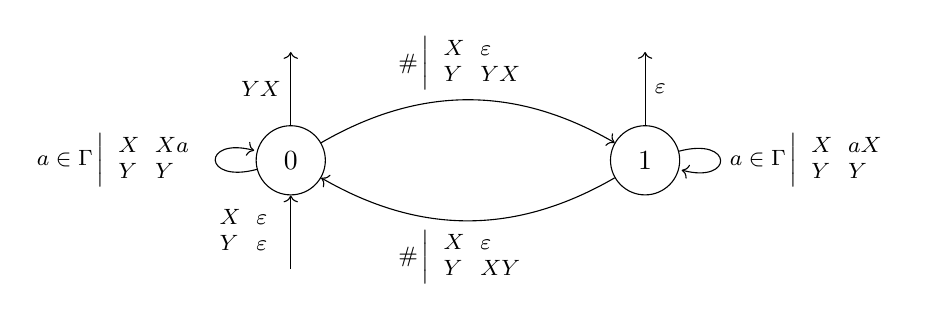
\begin{tikzpicture}[->,node distance=1.5cm]
    %[->,node distance=3.5cm,transform canvas={scale=1}]
    %every text node part/.style={font=\footnotesize}]
    \node[state] (A) {0} ;
    \node (D) [right of=A] {};
    \node (E) [right of=D] {};
    \node[state] (B) [right of=E] {1};
    \node (I) [below of=A] {};
    \node (OA) [above of=A] {};
    \node (OB) [above of=B] {};
  
  \path
    (I) edge node[left, style={font=\footnotesize}]
   {$\begin{array}{l@{~}c@{~}l} X &\regassign& \varepsilon \\ Y &\regassign& \varepsilon \end{array}$} (A) ;
  \path
    (A) edge node[left, style={font=\footnotesize}]
   {$YX$} (OA) ;
  \path
    (B) edge node[right, style={font=\footnotesize}]
   {$\varepsilon$} (OB) ;
  \path
    (A) edge [bend left] node[above, style={font=\footnotesize}]
   {$\#\left| \begin{array}{l@{~}c@{~}l} X &\regassign& \varepsilon \\ Y &\regassign& YX \end{array} \right.$} (B) ;
  \path (B) edge [loop right] node[right,style={font=\footnotesize}]
  {$a \in \Gamma \left| \begin{array}{l@{~}c@{~}l} X &\regassign& aX \\ Y &\regassign& Y \end{array} \right.$}
  (A) ;
  \path (B) edge [bend left] node[below,style={font=\footnotesize}]
   {$\#\left| \begin{array}{l@{~}c@{~}l} X &\regassign& \varepsilon \\ Y &\regassign& XY \end{array} \right.$}
  (A) ;
  \path (A) edge [loop left] node[left,style={font=\footnotesize}]
  {$a \in \Gamma \left| \begin{array}{l@{~}c@{~}l} X &\regassign& Xa \\ Y &\regassign& Y \end{array} \right.$}
  (A) ;
  \end{tikzpicture}
\end{center}
It computes the string-to-string function:
  \[
  \begin{array}{rcl!{\hspace{7em}} l}
  (\Gamma \sqcup \{ {\#} \})^* &\to& \Gamma^*
  & {(w_i \in \Gamma^*,\; (\Gamma \sqcup \{\#\})^* \cong \Gamma^*(\#\Gamma^*)^*)}\\
  w_0\#\ldots\#w_{2k} &\mapsto& \multicolumn{2}{l}{
    \ttreverse(w_{2k-1})
    \ttreverse(w_{2k-3})
    \ldots
    \ttreverse(w_1)
    w_0
    w_2
    \ldots
    w_{2k}} \\
  w_0\#\ldots\#w_{2k+1} &\mapsto& \varepsilon
  \end{array}
  \]
The SST starts out in the initial state $0$, with the initial values of $X$ and $Y$ both set to $\varepsilon$. At each transition, the new values of the registers are computed from the old ones by a parallel assignment. So for example, after reading $aab\#bbc$ (for $a,b,c\in\Gamma$), we are in state $1$ with the register contents $X = cbb$ and $Y = aab$. Finally, if the final state is $0$, the transducer outputs $(\text{final value of}\ Y)\cdot(\text{final value of}\ X)$; if the final state is $1$, it outputs the empty word.
\end{example}

Formally, a \emph{substitution} for the register set $R$ over the alphabet $\Gamma$ is a map $\sigma\colon R \to (\Gamma \cup R)^*$ (assuming that $R \cap \Gamma = \varnothing$). Typically, we have $\sigma(X) = Xa$ and $\sigma(Y) = Y$ for the leftmost register update in the state diagram of \Cref{ex:cecilia}. Substitutions \emph{compose}: define
\[ \sigma \substcomp \tau = (\text{the extension of}\ \sigma\ \text{to a monoid endomorphism of}\ (\Gamma \cup R)^*\ \text{fixing}\ \Gamma) \circ \tau \]
for $\sigma,\tau \colon R \to (\Gamma \cup R)^*$. There is some \enquote{contravariance} going on in this definition: even though we use $f \circ g$ to mean \enquote{apply $g$ then $f$} as usual, the register update specified by $\sigma\substcomp\tau$ corresponds to the update given by $\sigma$ followed by the one given by $\tau$. In other words, if we write $\sigma^\dagger \colon (\Gamma^*)^R \to (\Gamma^*)^R$ for the map between register values specified by $\sigma$ -- so in the above example, $\sigma^\dagger(\rho)(X) = \rho(X)\cdot a$ and $\sigma^\dagger(\rho)(Y) = \rho(Y)$ -- then $(\sigma\substcomp\tau)^\dagger = \tau^\dagger \circ \sigma^\dagger$.

To take into account the finite-state control, we consider the notion of \emph{substransition}: a map $\alpha \colon Q \to Q \times (R \to (\Gamma \cup R))^*$ where $Q$ is a set of states. Substransitions also compose (this is an instance of the wreath product construction):
\[ \text{for}\ q\in Q,\quad (\alpha\substcomp\beta)(q) = (q'',\sigma\substcomp\tau)\ \text{where}\ \alpha(q) = (q',\sigma)\ \text{and}\ \beta(q') = (q'',\tau) \]
\begin{definition}
  We write $\SubsTrans(Q,R,\Gamma)$ for the monoid of all substransitions over the set of states $Q$, the set of registers $R$ and the alphabet $\Gamma$, equipped with $\substcomp$.
\end{definition}
We first introduce \emph{copyful} streaming string transducers, which compute a strict superclass of the regular string functions~\cite{CopyfulSST}. Then we introduce the \emph{bounded-copy} restriction, which brings the computational power down to precisely the regular functions. Syntactically, this is a more permissive discipline than the \enquote{copyless} condition mentioned in the introduction; the equivalence between copyless and bounded-copy SSTs was established in\footnote{\tito{Finite coyping~\cite{MacroMSO} = bounded-copy~\cite{AlurFT12} (TODO: check)}
}~\cite[Section~IV.A]{AlurFT12}.

\begin{definition}
  \label{def:sst}
  A (deterministic copyful) \emph{streaming string transducer (SST)} with input
  alphabet $\Sigma$ and output alphabet $\Gamma$ is a tuple $\mathcal{T} = (Q, q_0, R,
  \delta, \vec{u}_I, F)$ where
\begin{itemize}
\item $Q$ is a finite set of \emph{states} and $q_0 \in Q$ is the \emph{initial
    state};
\item $R$ is a finite set of \emph{register names}, that we require to be
  disjoint from $\Gamma$;
\item $\delta \colon \Sigma \to \SubsTrans(Q,R,\Gamma)$ is the \emph{transition function};
\item $\vec{u}_I \in (\Sigma^*)^R$ describes the \emph{initial register values};
\item $F \colon Q \to (\Gamma \cup R)^*$ is the \emph{final output function}.
\end{itemize}
For an input word $w \in \Sigma^*$, the output of $\mathcal{T}$ is determined as follows. Let $(q,\sigma) = \delta^*(w)(q_0)$ where $\delta^*$ is the unique extension of $\delta$ to a monoid homomorphism $\Sigma^* \to \SubsTrans(Q,R,\Gamma)$. Apply $\sigma^\dagger \colon (\Gamma^*)^R \to (\Gamma^*)^R$ to $\vec{u}_I$ to get a tuple $\vec{v} = (v_X)_{X\in R}$ of final register values. Finally, replace each occurrence in $F(q)$ of a register name $X\in R$ by the corresponding value $v_X \in \Gamma^*$ to obtain an output string in $\Gamma^*$.
\end{definition}
\begin{definition}[see e.g.~{\cite{AlurFT12,AperiodicSST}}]
  A streaming string transducer whose transition function is $\delta \colon \Sigma \to \SubsTrans(Q,R,\Gamma)$ is \emph{bounded-copy} when there is some bound $k\in\mathbb{N}$ such that for every $q\in Q$, $w \in \Gamma^*$ and $X,Y\in R$, the string $\sigma(X)$ where $\delta^*(w)(q) = (q',\sigma)$ contains at most $k$ occurrences of~$Y$.
  In this paper, we take computability by bounded-copy SSTs as the definition of \emph{regular string-to-string functions}.
\end{definition}
The SST of \Cref{ex:cecilia} is bounded-copy (see \Cref{ex:cecilia-monoid} below). The following example of streaming string transducer is \emph{not} bounded-copy: it has a single state $q$ and a single register $X$; it performs $X \regassign XX$ for each input letter; the initial value is $X = a$ and the final output function is $F(q) = X$. This SST computes the function is $w \mapsto a\dots(2^{|w|}\ \text{times})\dots a$ which is not a regular function since its growth is not linearly bounded. Observe that the substitution $\sigma$ corresponding to an input factor $w$ is $\sigma \colon X \mapsto X\dots(2^{|w|}\ \text{times})\dots X$ -- this violates the bounded-copy condition.

The notion of bounded-copy SST can be rephrased using the monoid homomorphism $\tterase_\Gamma \colon \SubsTrans(Q,R,\Gamma) \to \SubsTrans(Q,R,\varnothing)$ which \enquote{erases all letters from $\Gamma$}, built by lifting the homomorphism $w \in \Gamma^* \mapsto \varepsilon \in \varnothing^*$ in the unique sensible way. 
\begin{proposition}\label{prop:bounded-copy-finiteness}
  An SST with transition function $\delta \colon \Sigma \to \SubsTrans(Q,R,\Gamma)$ is bounded-copy if and only if $\tterase_\Gamma(\delta^*(\Sigma^*))$ is a \emph{finite} submonoid of $\SubsTrans(Q,R,\varnothing)$. 
\end{proposition}
\begin{remark}
  This monoid $\tterase_\Gamma(\delta^*(\Sigma^*))$ is called the \emph{substitution transition monoid} of the given SST in~\cite[Section~3]{AperiodicSST}.
\end{remark}
\begin{example}\label{ex:cecilia-monoid}
  For the streaming string transducer of \Cref{ex:cecilia} (recall that its input alphabet is $\Gamma\cup\{\#\}$), we have (abbreviating $\ttreverse(w)$ by $\widetilde{w}$):
  \begin{align*}
    \text{for}\ w\in\Gamma^*,\; \delta^*(w) &= \begin{cases}
      0 \mapsto (0, (X \mapsto Xw \mid Y \mapsto Y))\\
      1 \mapsto (1, (X \mapsto \widetilde{w}X \mid Y \mapsto Y))
    \end{cases}\\
    \delta^*(w_0 \# \dots \# w_{2k+1}) &= \begin{cases}
      0 \mapsto (1, (X \mapsto \widetilde{w_{2k+1}} \mid Y \mapsto \widetilde{w_{2k-1}} \dots \widetilde{w_1} YX w_0 \dots w_{2k}))\\
      1 \mapsto (0, (X \mapsto w_{2k+1} \mid Y \mapsto \widetilde{w_{2k}} \dots \widetilde{w_0}XY w_1 \dots w_{2k-1}))
    \end{cases}\\
    \delta^*(w_0 \# \dots \# w_{2k+2}) &= \begin{cases}
      0 \mapsto (0, (X \mapsto w_{2k+2} \mid Y \mapsto \widetilde{w_{2k+1}} \dots \widetilde{w_1}YX w_0 \dots w_{2k}))\\
      1 \mapsto (1, (X \mapsto \widetilde{w_{2k+2}} \mid Y \mapsto \widetilde{w_{2k}} \dots \widetilde{w_0} XY w_1 \dots w_{2k+1}))
    \end{cases}
  \end{align*}
  By erasing the parts in $\Gamma^*$ of the right-hand sides, we see that the substitution transition monoid has three elements: the identity (which is the image of all words without $\#$) and
  \[ \begin{cases}
    0 \mapsto (1, (X \mapsto \varepsilon \mid Y \mapsto YX))\\
    1 \mapsto (0, (X \mapsto \varepsilon \mid Y \mapsto XY))
  \end{cases} \qquad\quad \begin{cases}
    0 \mapsto (0, (X \mapsto \varepsilon \mid Y \mapsto YX))\\
    1 \mapsto (1, (X \mapsto \varepsilon \mid Y \mapsto XY))
  \end{cases} \]
  Hence, since $3 < \infty$, the SST of \Cref{ex:cecilia} is bounded-copy.
\end{example}


\section{Register transducer semigroups}

We now introduce our first definition of regular semigroup-to-semigroup functions, heavily inspired by streaming string transducers. In the definition below, the maps $\mu_{s_1,s_2}$ should be understood as analogous to the substitutions in SSTs. At the same time, the whole definition itself can be seen at first as an abstraction of the monoid denoted by $\delta^*(\Sigma^*)$ in the previous section -- though we will see that even for string-to-string functions, we have good reasons to work with semigroups rather than monoids.

\begin{definition}
    A \emph{finitary semigroup with registers} $\mathcal{S}$ consists of a finite semigroup $S$, a family $(R_s)_{s\in S}$ of finite nonempty sets, and a family of functions
    \[ \mu_{s_1, s_2}\colon R_{s_1 s_2} \to (R_{s_1} + R_{s_2})^+ \quad\text{for}\ s_1, s_2 \in S\]
    such that for all $s_1, s_2, s_3 \in S$, the following associativity diagram
    commutes:
    \[\begin{tikzcd}
        [column sep=2.5cm]
        &
        (R_{s_1 s_2} + R_{s_3})^+
        \ar[r,"(\mu_{s_1,s_2}+\mathrm{id})^+"']
        &
        ((R_{s_1}+R_{s_2})+R_{s_3})^+
        \ar[dd,"\text{assoc.\ of}\ +"]
        \\
        R_{s_1 s_2 s_3}
        \ar[ur,"\mu_{s_1s_2,s_3}"]
        \ar[dr,"\mu_{s_1,s_2s_3}"']
        \\
        &
        (R_{s_1} + R_{s_2 s_3})^+
        \ar[r,"(\mathrm{id}+\mu_{s_2,s_3})^+"]
        &
        (R_{s_1}+(R_{s_2}+R_{s_3}))^+
      \end{tikzcd}\]
    For any semigroup $A$, we define $\mathcal{S}[A] = \displaystyle\bigcup_{s\in S} \{s\} \times A^{R_s}$
    endowed with the binary operation
    \[ (s_1,(a_{1,X})_{X\in R_{s_1}}) \cdot (s_2,(a_{2,Y})_{Y\in R_{s_2}}) = (s_1 s_2,\, (\overbrace{\mathrm{flatten}}^{\mathclap{A^+ \to A\ \text{using the semigroup operation in}\ A}} \circ \underbrace{\mathrm{substitute}}_{\mathclap{\text{replace each}\ X \in R_{s_1}\ \text{(resp.\ $Y \in R_{s_2}$) by}\ a_{1,X}\ \text{(resp.\ $a_{2,Y}$)}}} \circ \mu_{s_1 s_2}(Z))_{Z\in R_{s_1 s_2}}) \]
\end{definition}
\begin{proposition}
  For any finitary semigroup with registers $\mathcal{S}$ and any semigroup $A$, the binary operation on $\mathcal{S}[A]$ is associative: $\mathcal{S}[A]$ is a semigroup.
\end{proposition}
\begin{example}\label{ex:fsr-simple}
  Let $S = \{0,1\}$ with usual multiplication and $R_0 = R_1 = \{X,Y\}$. Let us write $\{X,Y\}+\{X,Y\}=\{X_{\mathrm{l}}, X_{\mathrm{r}}, Y_{\mathrm{l}}, Y_{\mathrm{r}}\}$ with $X_{\mathrm{l}}$ (resp.~$X_{\mathrm{r}}$) referring to the left (resp.~right) copy of $X$. The following definition of $\mu$ satisfies the associativity condition:
  \[ \forall i,j \in \{0,1\}, \qquad \mu_{i,j}(X) = X_{\mathrm{l}} X_{\mathrm{r}} \qquad \mu_{i,0}(Y) = X_{\mathrm{l}} Y_{\mathrm{r}} \qquad \mu_{i,1}(Y) = Y_{\mathrm{l}} Y_{\mathrm{r}} \]
  So $\mathcal{S} = (S,R,\mu)$ is a finitary semigroup with registers. We have for example in $\mathcal{S}[(\mathbb{N},+)]$
  \[ (1,(X\mapsto42\mid Y\mapsto218)) \cdot (0,(X\mapsto1\mid Y\mapsto100)) = (0,(X\mapsto43\mid Y\mapsto142)) \]
\end{example}

\begin{definition}\label{def:reg-trans-semigroup}
    A \emph{register transducer semigroup} consists of a finitary semigroup with registers $\mathcal{S} = (S,R,\mu)$ together with a family of strings $\omega_s \in (R_s)^+$ for $s\in S$.

    A function $f\colon A \to B$ between semigroups is said to be \emph{recognized} by $(\mathcal{S}, \omega)$ if it admits a decomposition $f = \outfun_B \circ h$ where $h \colon A \to \mathcal{S}[B]$ is some semigroup homomorphism and
    \[ \outfun_B(s,(b_X)_{X \in R_s}) = \mathrm{flatten}(\text{replace each}\ X\in R_s\ \text{in}\ \omega_s\ \text{by}\ b_X) \]
    $f$ is called \emph{regular} when there exists a register transducer semigroup that recognizes it.
\end{definition}
\begin{example}\label{ex:rts-simple}
  Let $\mathcal{S}$ be the finitary semigroup with registers from \Cref{ex:fsr-simple}. Reusing the notations from that example, let us choose $\omega_0 = \omega_1 = Y$; this makes $(\mathcal{S},\omega)$ is a register transducer semigroup. It can recognize the function $f\colon \{a,b,c\}^* \to \{a,b\}^*$ such that
  \[ \forall u \in \{a,b,c\}^*,\;\forall v \in \{a,b\}^*,\quad f(ucv) = a^{|u|}bv \quad\text{and}\quad f(v) = v \]
  (inspired by~\cite[Theorem~5.6]{MacroMSO}). Indeed, to do so, we pick the semigroup homomorphism
  \[ h\colon w \in \{a,b,c\}^* \mapsto ((1\ \text{if}\ w\in\{a,b\}^*,\;\text{else}\ 0),\; (X\mapsto a^{|w|} \mid Y \mapsto f(w)) \in \mathcal{S}[\{a,b\}^*]\]
\end{example}

\begin{theorem}
  A function between free monoids is regular in the sense of \Cref{def:reg-trans-semigroup} (i.e.\ recognized by some register transducer semigroup) if and only if it is a regular string function in the conventional sense (i.e.\ computed by some bounded-copy SST).
\end{theorem}
\begin{proof}
  We first treat \enquote{only if}, then \enquote{if}.

  \proofsubparagraph{From a register transducer semigroup to a bounded-copy streaming string transducer.}
  Let $(\mathcal{S}=(S,R,\mu),\,\omega)$ be a register transducer semigroup and $h\colon \Sigma^* \to \mathcal{S}[\Gamma^*]$ be a semigroup homomorphism. We want a bounded-copy SST that computes $\outfun_{\Gamma^*}\circ h$. Our solution will be to take an \enquote{obvious choice} of SST, which clearly computes this function -- the idea is that the configuration (state + register contents) of the SST, after reading an input prefix $w\in\Sigma^*$, represents $h(w)$ -- and then check that it is bounded-copy.
  \begin{itemize}
    \item The set of states is $Q = S$ and the initial state is the first component of $h(\varepsilon)$. (Note that while $\mathcal{S}[\Gamma^*]$ is not necessarily a monoid, $h(\Sigma^*)$ always is, with $h(\varepsilon)$ as its unit element.)
    \item The registers are $R = \displaystyle\bigcup_{s\in S} R_s$ (without loss of generality, we take the $R_s$ pairwise disjoint).
    \item For $c\in\Sigma$ and $q\in Q=S$, we define $\delta(c)(q) = (qs,\sigma)$ where $(s, (v_X)_{X\in R_s}) = h(c)$ and
    \[ \sigma\colon Y \in R ~~\mapsto~~ \begin{cases}
      \text{replace each}\ X \in R_s\ \text{by}\ v_X\ \text{in}\ \mu_{q,s}(Y) & \text{when}\ Y \in R_{qs}\\
      \varepsilon & \text{otherwise}
    \end{cases} \]
    \item The initial register values are $X:=u_{0,X}$ for any $X\in R_{q_0}$ where $(q_0,(u_{0,X})_{X\in R_{q_0}}) = h(\varepsilon)$, and $X := \varepsilon$ for other registers.
    \item The final output function is $q \mapsto \omega_q$.
  \end{itemize}
  One can verify that $\tterase_\Gamma(\delta^*(w))(q) = (qs, [\text{something fully determined by}\ \mu_{q,s}])$ where $s$ is the 1st component of $h(w)$ for any $w\in\Sigma^*$ and $q\in Q$. Since $s$ lives in the finite semigroup~$S$, the monoid $\tterase_\Gamma(\delta^*(\Sigma^*))$ is finite. By \Cref{prop:bounded-copy-finiteness}, our SST is bounded-copy.

  \proofsubparagraph{From a bounded-copy streaming string transducer to a register transducer semigroup.}

  We start by illustrating the main idea on the SST of \Cref{ex:cecilia}. This SST has several convenient properties that simplify the construction (in particular, the semigroup that we get is a monoid): all its registers are initialized with $\varepsilon$, and the final output function merely combines registers without adding letters from the output alphabet. We will see later how to handle the minor complications that may arise without these properties.
  \begin{claim}
    The function $\Sigma^* \to \Gamma^*$ (with $\Sigma = \Gamma\cup\{\#\}$) of \Cref{ex:cecilia} is recognized by a register transducer semigroup $(\mathcal{M} = (M,R,\mu),\; \omega)$, where $M = \tterase_\Gamma(\delta^*(\Sigma^*))$ is the finite substitution transition monoid described in \Cref{ex:cecilia-monoid}, and such that the infinite monoid $\delta^*(\Sigma^*)$ can be identified with a submonoid of $\mathcal{M}[\Gamma^*]$.
  \end{claim}
  \begin{claimproof}[Proof sketch]
    We shall work with the following abbreviations for $u,v,\ldots \in \Sigma^*$:
    \begin{align*}
      \alpha[u,v] &= \begin{cases}
        0 \mapsto (0, (X \mapsto Xu \mid Y \mapsto Y))\\
        1 \mapsto (1, (X \mapsto vX \mid Y \mapsto Y))
      \end{cases}\\
      \text{for}\ i \in \{0,1\},\quad \beta_i[u_1,\dots,v_3] &= \begin{cases}
        0 \mapsto (i,\quad\;\; (X \mapsto u_1 \mid Y \mapsto u_2 YX u_3))\\
        1 \mapsto (1-i, (X \mapsto v_1 \mid Y \mapsto v_2 XY v_3))
      \end{cases}      
    \end{align*}
    We also write $\alpha = \alpha[\varepsilon,\varepsilon]$ and $\beta_i = \beta_i[\varepsilon,\dots,\varepsilon]$.
    Note that $M = \{\alpha,\beta_0,\beta_1\}$ (equipped with composition of substransitions), while every element of $\delta^*(\Sigma^*)$ is of the form $\alpha[\dots]$ or $\beta_i[\dots]$. The set $\mathfrak{M}$ of all $\alpha[\dots]$ and $\beta_i[\dots]$ is a submonoid of $\SubsTrans(\{0,1\},\{X,Y\},\Gamma)$, since $\alpha$ is the unit element and we have composition equations such as
    \[ \alpha[u,v] \cdot \beta_1[u_1,u_2,u_3,v_1,v_2,v_3] = \beta_1[u_1,u_2,(u \cdot u_3),v_1,(v_2 \cdot v),v_3] \]
    The idea is then to define $\mathcal{M} = (M,R,\mu)$ in such a way that $\mathfrak{M} \cong \mathcal{M}[\Gamma^*]$. For the registers, we take $R_\alpha = \{U,V\}$ and $R_{\beta_i} = \{U,V\} \times \{1,2,3\}$. This allows us to define a bijection
    \begin{align*}
      \mathcal{M}[\Gamma^*] &\to \mathfrak{M}\\
      (\alpha, (w_{U}, w_{V})) &\mapsto \alpha[w_{U},w_{V}]\\
      (\beta_i, (w_{U,1},\dots,w_{V,3})) &\mapsto \beta_i[w_{U,1},\dots,w_{V,3}]
    \end{align*}
    Observe also that for $\lambda,\gamma\in\{\alpha,\beta_0,\beta_1\}$, we have $\lambda[\dots] \cdot \gamma[\dots] = (\lambda\cdot\gamma)[\dots]$, which brings us halfway to having the above bijection be a monoid isomorphism. To get there, there remains to choose a definition of $\mu$ reflecting the composition equations; for example the above one concerning $\alpha$ and $\beta_1$ leads us to define $\mu_{\alpha,\beta_1}$ as
    \[ (U,1)\mapsto(U,1) \mid \dots \mid (U,3) \mapsto U \cdot (U,3) \mid \dots \mid (V,2) \mapsto (V,2) \cdot V \mid (V,3) \mapsto (V,3) \]
    We set the output strings of our register transducer semigroup according to the initial state and final output function of \Cref{ex:cecilia}, as follows:
    \begin{itemize}
      \item $\omega_\alpha = U$ because after applying $\alpha[u,v]$ to the initial configuration of the SST, we are in state 0, $X = u$ \& $Y = \varepsilon$, and the final output function tells us to output $YX = u$;
      \item $\omega_{\beta_0} = (U,2)\cdot(U,3)\cdot(U,1)$ because after applying $\beta_0[u_1,\dots,v_3]$ to the initial configuration, we are in state 0 and $X$ contains $u_1$ while $Y$ contains $u_2 u_3$;
      \item $\omega_{\beta_1} = \varepsilon$ because applying $\beta_1[\dots]$ to the initial configuration brings us in state 1, in which the final output function tells us to output $\varepsilon$.
    \end{itemize}
    Finally, to recognize the function of \Cref{ex:cecilia}, we use the semigroup homomorphism $(\text{inverse of above isomorphism}\ \mathcal{M}[\Gamma^*] \to \mathfrak{M}) \circ \delta^* : \Sigma^* \to \mathcal{M}[\Gamma^*]$ -- indeed $\delta^*(\Sigma^*) \subset \mathfrak{M}$.
  \end{claimproof}

  \tito{todo when $f(\varepsilon) \neq \varepsilon$}
\end{proof}



\section{Functorial transducer semigroups and warm-up theorems}

\tito{Exactly like \Cref{sec:warm-up}}

\section{Finiteness-preserving functors define regular functions}


\subsection{From registers to functors}

\tito{todo}

\begin{remark}
  This data induces the finite polynomial functor from semigroups to sets BLAH  
  which can be turned into a functor from semigroups to semigroups thanks to $\mu$.


    Equivalently, consider the following symmetric monoidal category:
    \begin{description}
        \item[Objects:] finite polynomial functors (in one variable).
        \item[Morphisms:] natural transformations.
        \item[Monoidal product:] pointwise cartesian product of sets.
    \end{description}
    A finitary semigroup with registers is the same thing as a \enquote{semigroup object} (defined by removing the unit requirement from monoid objects) in this monoidal category of finite polynomial functors.

    \tito{Blah is equivalent to specifying a natural transformation from the associated polynomial functor to the forgetful functor from semigroups to sets, so it induces a functorial transducer semigroup in the expected way.}
\end{remark}


\begin{remark}
This should also work if we have a single finite nonempty set of registers $R$ for all semigroup elements instead of a family $(R_s)_{s\in S}$ though the equivalence proof is slightly less immediate for semigroups than for monoids (you need to use the output function to produce \enquote{default} elements with which to fill unused registers). Note that the \enquote{substitution transition monoid} operation \enquote{naturally} produces something with a varying register set.

Another possible variation on the definition is to have a choice of output register for each element of the control semigroup: $r_s \in R_s$ for $s\in S$ instead of $\omega_s \in (R_s)^+$. This does not decrease the expressivity of the model.
\end{remark}


\subsection{From functors to registers}

\begin{theorem}
  For every finiteness-preserving functorial transducer semigroup $(\functor, \outfun)$, there is another one $(\functor',\outfun')$
  \begin{itemize}
    \item which is induced by some register transducer semigroup,
    \item and which admits a natural transformation $\eta \colon \functor \Rightarrow \functor'$ such that $\outfun = \outfun' \circ \eta$.
  \end{itemize}
  Hence every function recognized by $(\functor,\outfun)$ is also recognized by $(\functor',\outfun')$ (by the second item) and thus is regular (by the first item).
\end{theorem}
\begin{proof}
    Let $(\functor,\outfun)$ be a functorial transducer semigroup, and suppose $\functor$ preserves finiteness, so $\functor1$ is finite. We first build a finitary semigroup with registers that doesn't entirely fulfill our objectives, but still contains the core mechanism: $S = \functor1$, and for $s\in S$,
    \[ R_s = \sum_{l,r \in F(1)} \{\text{occurrences of}\ \mathtt{m}\ \text{in}\ (\text{factorized output of}\ (l,s,r)) \in 1\oplus1\oplus1 \cong \{\mathtt{l,m,r}\}^+\} \]
    For $s_1,s_2\in S$ we must now define a map $R_{s_1 s_2} \to (R_{s_1} + R_{s_2})^+$ describing the register recombination during a product. We derive it from the correspondence between
    \begin{itemize}
        \item the occurrences of $\mathtt{m}$ in the factorized output of $l \cdot (s_1 s_2)\cdot r$
        \item and the maximal factors in $\{\mathtt{m_1,m_2}\}^+$ inside
        \[ (\text{factorized output of}\ (l,s_1,s_2,r)) \in 1\oplus1\oplus1\oplus1 \cong \{\mathtt{l,m_1,m_2,r}\}^+ \]
    \end{itemize}
    Indeed, the morphism $1\oplus\mathop{!}\oplus1$ where $! \colon 1\oplus1 \to 1$ is the terminal morphism sends the maximal factors in $\{\mathtt{m_1,m_2}\}^+$ to $\mathtt{m}$ and is the identity on $\mathtt{l,r}$. To see that applying this to the factorized output of $(l,s_1,s_2,r)$ indeed yields the factorized output of $(l,s_1s_2,r)$, apply \Cref{lem:merge-middle} to $A=B=C=1$.

    We must also check that this operation is \enquote{associative}. For this, consider the factorized output of $(l,s_1,s_2,s_3,r)$ \ldots{}
    \tito{TODO above}

    Finally we define $\widehat\eta \colon \functor \Rightarrow \functorg$ where $\functorg$ is the functor induced by our semigroup with registers. For any $x \in \functor A$, apply $\functor! \colon \functor A \to \functor 1$ to get some $s \in S$. Then look at the factorized output of $(l,x,r)$ in $1\oplus A \oplus 1$ for each $(l,r)\in (\functor1)^2$ to get register values in $A^{R_s}$.

    The issue is that the output function for $\functor$ may not factor through $\widehat\eta$. To remediate that, we consider instead another semigroup with registers, inducing the functor $\functor'$, with the same underlying semigroup $S=\functor1$ and bigger register sets
    \[ R'_s = \{\bullet\} + R^{\mathrm{left}}_s + R^{\mathrm{right}}_s + R_s \quad\text{for}\ s\in S\]
    where $R^{\mathrm{left}}_s$ is the sum over $r \in \functor1$ of the sets of occurrences of $\mathtt{l}$ in the factorized output of $(s,r)$ which is in $1\oplus1\cong\{\mathtt{l,r}\}^+$, etc. Thus
    \[ \functor'A \cong \sum_{s\in S} A \times A^{R^{\mathrm{left}}_s} \times \dots \cong A \times \sum_{s\in S} A^{R^{\mathrm{left}}_s} \times \dots \]
    and we have then: $\outfun_A = (\text{left projection on}\ A) \circ \eta$ for the definition of $\eta$ extending $\widehat\eta$ in the obvious way.
\end{proof}

\begin{lemma}\label{lem:merge-middle}
    Let $A,B,C$ be semigroups. The following diagram commutes:
    \[\begin{tikzcd}
        [column sep=3cm]
        \functor A \times \functor B\times \functor B \times \functor C
        \ar[r,"\text{factorized output}"]
        \ar[d,"\functor A \times (\text{semigroup operation}) \times \functor C"']
        &
        A \oplus B \oplus B \oplus C
        \ar[d,"A \oplus (\mathrm{id}_B\,\text{or}\,\mathrm{id}_B) \oplus C"]
        \\
        \functor A \times \functor B \times \functor C
        \ar[r,"\text{factorized output}"]
        &
        A \oplus B \oplus C
    \end{tikzcd}\]
\end{lemma}
\tito{similar to \Cref{claim:merge-factorized-output}}
\begin{proof}
    By rotating the above diagram, we see that it corresponds to the outer rectangle in the following diagram (where we have expanded the definition of the factorized output functions, and used the associativity of 4-fold multiplication):
    \[\begin{tikzcd}
        [column sep=4cm]
        \functor A \times \functor B\times \functor B \times \functor C
        \ar[d,"\functor(\text{co-projection})^4"']
        \ar[r,"\functor A \times (\text{semigroup op}) \times \functor C"]
        &
        \functor A \times \functor B \times \functor C
        \ar[d,"\functor(\text{co-projection})^3"]
        \\
        \functor(A \oplus B \oplus B \oplus C)^4
        \ar[d,"\text{multiply middle two together}"']
        &
        \functor(A \oplus B \oplus C)^3
        \ar[dd,""]
        \\
        \functor(A \oplus B \oplus B \oplus C)^3
        \ar[d,"\text{semigroup operation}"']
        \ar[ru,"F(A \oplus (\mathrm{id}_B\,\text{or}\,\mathrm{id}_B) \oplus C)^3"']
        \\
        \functor(A \oplus B \oplus B \oplus C)
        \ar[d, "\outfun_{A \oplus B \oplus B \oplus C}"']
        \ar[r,"F(A \oplus (\mathrm{id}_B\,\text{or}\,\mathrm{id}_B) \oplus C)"]
        &
        \functor(A \oplus B \oplus C)
        \ar[d, ""]
        \\ 
        A \oplus B \oplus B \oplus C
        \ar[r,"A \oplus (\mathrm{id}_B\,\text{or}\,\mathrm{id}_B) \oplus C"]
        &
        A \oplus B \oplus C
    \end{tikzcd}\]
    The lower rectangle commutes by naturality of the output function. The middle trapeze commutes because of the homomorphism property of $F(A \oplus (\mathrm{id}_B\,\text{or}\,\mathrm{id}_B) \oplus C)$. Concerning the upper trapeze, it can be decomposed as the functor $(\cdots \times \cdots \times \cdots)$ applied to three diagrams that we can analyze independently. The first of those is
    \[\begin{tikzcd}
        [column sep=4cm]
        \functor A
        \ar[d,"\functor(\text{co-projection})"']
        \ar[r,"\mathrm{id}_A"]
        &
        \functor A
        \ar[d,"\functor(\text{co-projection})"]
        \\
        \functor(A \oplus B \oplus B \oplus C)
        \ar[d,"\mathrm{id}"']
        &
        \functor(A \oplus B \oplus C)
        \\
        \functor(A \oplus B \oplus B \oplus C)
            \ar[ru,"F(A \oplus (\mathrm{id}_B\,\text{or}\,\mathrm{id}_B) \oplus C)"']
    \end{tikzcd}\]
    By functoriality of $\functor$, the commutativity of this diagram reduces to
    \[ (\mathrm{id}_A \oplus \dots) \circ (\text{co-projection of}\ A\ \text{into}\ A\oplus(B\oplus B\oplus C)) = \text{co-projection of}\ A\ \text{into}\ A\oplus(B\oplus C) \]
    which is an elementary property of the coproduct $\oplus$ in any category (indeed the bifunctor structure of $\oplus$ is built using a coparing, which \enquote{cancels out} with the coprojection).
    Among the 3 diagrams that were combined by a 3-fold cartesian product, another one is identical to the above, with $C$ replacing $A$. There remains this one, in which we have added some parts in the middle:
    \[\begin{tikzcd}
        [column sep=2.5cm]
        \functor B\times \functor B
        \ar[d,"\functor(\text{co-proj})^2"']
        \ar[dr,"\functor(\text{co-proj})^2"]
        \ar[rr,"\text{semigroup operation}"]
        &
        &
        \functor B
        \ar[d,"\functor(\text{co-proj})"]
        \\
        \functor(A \oplus B \oplus B \oplus C)^2
        \ar[d,"\text{semigroup op}"']
        \ar[r,"h\times h"']
        &
        \functor(A \oplus B \oplus C)^2
        \ar[r,"\text{semigroup op}"]
        &
        \functor(A \oplus B \oplus C)
        \\
        \functor(A \oplus B \oplus B \oplus C)
            \ar[rru,"h = F(A \oplus (\mathrm{id}_B\,\text{or}\,\mathrm{id}_B) \oplus C)"']
    \end{tikzcd}\]
    The upper right trapeze commutes because $\functor$ applied to the co-projection of $B$ into $A\oplus B\oplus C$ is a homomorphism. The lower triangle commutes because $h$ is a homomorphism. Finally, the small upper left triangle can be shown to commute using the functoriality of $\functor$ followed by properties of the coproduct.
\end{proof}

\section{Conclusion}

\tito{Extension to forest algebra, etc.}

\end{document}
